% Options for packages loaded elsewhere
\PassOptionsToPackage{unicode}{hyperref}
\PassOptionsToPackage{hyphens}{url}
%
\documentclass[
  american,
  ,man,floatsintext]{apa6}
\title{Non-word repetition in children learning Yélî Dnye}
\author{Alejandrina Cristia\textsuperscript{1} \& Marisa Casillas\textsuperscript{2,3}}
\date{}

\usepackage{amsmath,amssymb}
\usepackage{lmodern}
\usepackage{iftex}
\ifPDFTeX
  \usepackage[T1]{fontenc}
  \usepackage[utf8]{inputenc}
  \usepackage{textcomp} % provide euro and other symbols
\else % if luatex or xetex
  \usepackage{unicode-math}
  \defaultfontfeatures{Scale=MatchLowercase}
  \defaultfontfeatures[\rmfamily]{Ligatures=TeX,Scale=1}
\fi
% Use upquote if available, for straight quotes in verbatim environments
\IfFileExists{upquote.sty}{\usepackage{upquote}}{}
\IfFileExists{microtype.sty}{% use microtype if available
  \usepackage[]{microtype}
  \UseMicrotypeSet[protrusion]{basicmath} % disable protrusion for tt fonts
}{}
\makeatletter
\@ifundefined{KOMAClassName}{% if non-KOMA class
  \IfFileExists{parskip.sty}{%
    \usepackage{parskip}
  }{% else
    \setlength{\parindent}{0pt}
    \setlength{\parskip}{6pt plus 2pt minus 1pt}}
}{% if KOMA class
  \KOMAoptions{parskip=half}}
\makeatother
\usepackage{xcolor}
\IfFileExists{xurl.sty}{\usepackage{xurl}}{} % add URL line breaks if available
\IfFileExists{bookmark.sty}{\usepackage{bookmark}}{\usepackage{hyperref}}
\hypersetup{
  pdftitle={Non-word repetition in children learning Yélî Dnye},
  pdfauthor={Alejandrina Cristia1 \& Marisa Casillas2,3},
  pdflang={en-US},
  pdfkeywords={phonology, non-word repetition, Papuan, non-industrial, non-urban, comparative, typology, markedness, literacy},
  hidelinks,
  pdfcreator={LaTeX via pandoc}}
\urlstyle{same} % disable monospaced font for URLs
\usepackage{graphicx}
\makeatletter
\def\maxwidth{\ifdim\Gin@nat@width>\linewidth\linewidth\else\Gin@nat@width\fi}
\def\maxheight{\ifdim\Gin@nat@height>\textheight\textheight\else\Gin@nat@height\fi}
\makeatother
% Scale images if necessary, so that they will not overflow the page
% margins by default, and it is still possible to overwrite the defaults
% using explicit options in \includegraphics[width, height, ...]{}
\setkeys{Gin}{width=\maxwidth,height=\maxheight,keepaspectratio}
% Set default figure placement to htbp
\makeatletter
\def\fps@figure{htbp}
\makeatother
\setlength{\emergencystretch}{3em} % prevent overfull lines
\providecommand{\tightlist}{%
  \setlength{\itemsep}{0pt}\setlength{\parskip}{0pt}}
\setcounter{secnumdepth}{-\maxdimen} % remove section numbering
% Make \paragraph and \subparagraph free-standing
\ifx\paragraph\undefined\else
  \let\oldparagraph\paragraph
  \renewcommand{\paragraph}[1]{\oldparagraph{#1}\mbox{}}
\fi
\ifx\subparagraph\undefined\else
  \let\oldsubparagraph\subparagraph
  \renewcommand{\subparagraph}[1]{\oldsubparagraph{#1}\mbox{}}
\fi
\newlength{\cslhangindent}
\setlength{\cslhangindent}{1.5em}
\newlength{\csllabelwidth}
\setlength{\csllabelwidth}{3em}
\newlength{\cslentryspacingunit} % times entry-spacing
\setlength{\cslentryspacingunit}{\parskip}
\newenvironment{CSLReferences}[2] % #1 hanging-ident, #2 entry spacing
 {% don't indent paragraphs
  \setlength{\parindent}{0pt}
  % turn on hanging indent if param 1 is 1
  \ifodd #1
  \let\oldpar\par
  \def\par{\hangindent=\cslhangindent\oldpar}
  \fi
  % set entry spacing
  \setlength{\parskip}{#2\cslentryspacingunit}
 }%
 {}
\usepackage{calc}
\newcommand{\CSLBlock}[1]{#1\hfill\break}
\newcommand{\CSLLeftMargin}[1]{\parbox[t]{\csllabelwidth}{#1}}
\newcommand{\CSLRightInline}[1]{\parbox[t]{\linewidth - \csllabelwidth}{#1}\break}
\newcommand{\CSLIndent}[1]{\hspace{\cslhangindent}#1}
\usepackage{fontspec}

\setmainfont{Doulos SIL} % Set main font to Doulos SIL
% Manuscript styling
\usepackage{upgreek}
\captionsetup{font=singlespacing,justification=justified}

% Table formatting
\usepackage{longtable}
\usepackage{lscape}
% \usepackage[counterclockwise]{rotating}   % Landscape page setup for large tables
\usepackage{multirow}		% Table styling
\usepackage{tabularx}		% Control Column width
\usepackage[flushleft]{threeparttable}	% Allows for three part tables with a specified notes section
\usepackage{threeparttablex}            % Lets threeparttable work with longtable

% Create new environments so endfloat can handle them
% \newenvironment{ltable}
%   {\begin{landscape}\centering\begin{threeparttable}}
%   {\end{threeparttable}\end{landscape}}
\newenvironment{lltable}{\begin{landscape}\centering\begin{ThreePartTable}}{\end{ThreePartTable}\end{landscape}}

% Enables adjusting longtable caption width to table width
% Solution found at http://golatex.de/longtable-mit-caption-so-breit-wie-die-tabelle-t15767.html
\makeatletter
\newcommand\LastLTentrywidth{1em}
\newlength\longtablewidth
\setlength{\longtablewidth}{1in}
\newcommand{\getlongtablewidth}{\begingroup \ifcsname LT@\roman{LT@tables}\endcsname \global\longtablewidth=0pt \renewcommand{\LT@entry}[2]{\global\advance\longtablewidth by ##2\relax\gdef\LastLTentrywidth{##2}}\@nameuse{LT@\roman{LT@tables}} \fi \endgroup}

% \setlength{\parindent}{0.5in}
% \setlength{\parskip}{0pt plus 0pt minus 0pt}

% \usepackage{etoolbox}
\makeatletter
\patchcmd{\HyOrg@maketitle}
  {\section{\normalfont\normalsize\abstractname}}
  {\section*{\normalfont\normalsize\abstractname}}
  {}{\typeout{Failed to patch abstract.}}
\patchcmd{\HyOrg@maketitle}
  {\section{\protect\normalfont{\@title}}}
  {\section*{\protect\normalfont{\@title}}}
  {}{\typeout{Failed to patch title.}}
\makeatother
\shorttitle{NWR in Yélî Dnye learners}
\keywords{phonology, non-word repetition, Papuan, non-industrial, non-urban, comparative, typology, markedness, literacy\newline\indent Word count: ~12,200 words}
\usepackage{lineno}

\linenumbers
\usepackage{csquotes}
\ifXeTeX
  % Load polyglossia as late as possible: uses bidi with RTL langages (e.g. Hebrew, Arabic)
  \usepackage{polyglossia}
  \setmainlanguage[variant=american]{english}
\else
  \usepackage[main=american]{babel}
% get rid of language-specific shorthands (see #6817):
\let\LanguageShortHands\languageshorthands
\def\languageshorthands#1{}
\fi
\ifLuaTeX
  \usepackage{selnolig}  % disable illegal ligatures
\fi


\affiliation{\vspace{0.5cm}\textsuperscript{1} Laboratoire de Sciences Cognitives et de Psycholinguistique, Département d'Etudes Cognitives, ENS, EHESS, CNRS, PSL University\\\textsuperscript{2} Max Planck Institute for Psycholinguistics\\\textsuperscript{3} University of Chicago}

\abstract{
In non-word repetition (NWR) studies, participants are presented auditorily with an item that is phonologically legal but lexically meaningless in their language, and asked to repeat this item as closely as possible. NWR scores are thought to reflect some aspects of phonological development, saliently a perception-production loop supporting flexible production patterns. In this study, we report on NWR results among children (N = 40, aged 3--10 years) learning Yélî Dnye, an isolate language spoken on Rossel Island in Papua New Guinea. Results make three contributions that are specific, and a fourth that is general. First, we found that non-word items containing typologically frequent sounds are repeated without changes more often than non-words containing typologically rare sounds, above and beyond any within-language frequency effects. Second, we documented rather weak effects of item length. Third, we found that NWR scores correlate strongly with age, whereas they are only weakly correlated with child sex, maternal education, and birth order. Fourth, we weave our results with those of others to serve the general goal of reflecting on how NWR scores can be compared across participants, studies, languages, and populations, and the extent to which they shed light on the factors universally structuring variation in phonological development at a global and individual level.
}



\begin{document}
\maketitle

\hypertarget{introduction}{%
\subsection{Introduction}\label{introduction}}

Children's perception and production of phonetic and phonological units continues developing well beyond the first year of life, even extending into middle childhood (e.g., Hazan \& Barrett, 2000; Rumsey, 2017). Some of the evidence for later phonological development comes from non-word repetition (NWR) tasks. In the present study, we use NWR to investigate the phonological development of children learning Yélî Dnye, an isolate language spoken in Papua New Guinea (PNG), which has a large and unusually dense phonological inventory. This allows us to contribute data at the intersection of language typology, language acquisition, and individual variation, as presented in more detail below.

\hypertarget{defining-nwr}{%
\subsubsection{Defining NWR}\label{defining-nwr}}

In a basic NWR task, the participant listens to a production of a word-like form, such as /bilik/, and then repeats back what they heard without changing any phonological feature that is contrastive in the language. For instance, in English, a response of {[}bilig{]} or {[}pilik{]} would be scored as incorrect; a response {[}biːlik{]}, where the vowel is lengthened without change of quality would be scored as correct, because English does not have contrastive vowel length.

NWR has been used to seek answers to a variety of theoretical questions, including what the links between phonology, working memory, and the lexicon are (Bowey, 2001), and how extensively phonological constraints found in the lexicon affect online production (Gallagher, 2014). NWR is also frequently used in applied contexts, notably as a diagnostic tool for language delays and disorders (Chiat, 2015; Estes, Evans, \& Else-Quest, 2007). Since non-words can be generated in any language, it has attracted the attention of researchers working in multilingual and linguistically diverse environments, particularly in Europe in the context of diagnosing language impairments among bilingual children (Armon-Lotem, Jong, \& Meir, 2015; Chiat, 2015; COST Action, 2009; Meir, Walters, \& Armon-Lotem, 2016). NWR tasks probably tap into many skills (for relevant discussion see Coady \& Evans, 2008; Santos, Frau, Labrevoit, \& Zebib, 2020). Non-words can be designed to try to isolate certain skills more narrowly; for instance, one can choose non-words that contain real morphemes in order to load more on prior language experience, or non-words that are shorter to avoid loading on working memory (see a discussion in Chiat, 2015). Broadly, however, NWR scores will necessarily reflect to a certain extent phonological knowledge (to perceive the item precisely despite not having heard it before) as well as online phonological working memory (to encode the item in the interval between hearing it and saying it back) and flexible production patterns (to produce the item precisely despite not having pronounced it before).

\hypertarget{the-present-work}{%
\subsubsection{The present work}\label{the-present-work}}

We aimed to contribute to four areas of research. We motivate each in turn.

\hypertarget{nwr-and-typology}{%
\paragraph{NWR and typology}\label{nwr-and-typology}}

The first research area is at the intersection of typology and phonological development. There has been an interest in adapting NWR to different languages, in part for applied purposes. In a review of NWR as a potential task to diagnose language impairments among bilingual children in Europe, Chiat (2015) discusses the impossibility of creating language-universal non-word items: Languages vary in their phonological inventory, sound sequencing (phonotactics), syllable structure, and word-level prosody. As a result, any one item created will be relatively easier if it more closely resembles real words in a language, making it difficult to balance difficulty when comparing children learning different languages. This previous literature also suggests some dimensions of difficulty---an issue to which we return in the next subsection.

Although this cross-linguistic literature is rich, the potential difficulty associated with specific phonetic targets composing the non-words has received relatively little attention. For example, Chiat (2015) discusses segmental complexity as a function of whether there are consonant clusters -- which is arguably a factor reflecting phonotactics and syllable structure.

In the present study, we thought it was relevant to represent the rich phonological inventory found in Yélî Dnye, by including a variety of phonetic targets. Some of them are cross-linguistically rare, in that they are less common across languages than other sounds or phonetic targets. Phonologists, phoneticians, and psycholinguists have discussed the extent to which cross-linguistic frequency may reflect ease of processing and acquisition via diachronic language change. These works focus largely on phonotactics (Moreton \& Pater, 2012), perceptual parsing of the (ambiguous) linguistic signal (Beddor, 2009; Ohala, 1981), and individual differences in processing styles (Bermúdez-Otero, 2015); which are small effects that may nonetheless cumulatively drive language change via phonologization (see Yu, 2021 for a recent review). Thus, the correlation between typological frequency and ease of acquisition is typically assumed to emerge from one or more of the following causal paths:

\begin{enumerate}
\def\labelenumi{\arabic{enumi}.}
\tightlist
\item
  Sounds (and sound sequences) that are harder to perceive tend to be misperceived and thus lost diachronically
\item
  Sounds (and sound sequences) that are harder to pronounce tend to be mispronounced and thus lost diachronically
\item
  Sound sequences that are harder to hold in memory tend to be mispronounced and thus lost diachronically
\end{enumerate}

Since NWR can tap into perception, production, and working memory, we predicted that variation in NWR across items will correlate with the cross-linguistic frequency of the phones composing those items.

\hypertarget{length-effects-on-nwr}{%
\paragraph{Length effects on NWR}\label{length-effects-on-nwr}}

The second research area we contribute data to is research looking at the impact of word length on NWR repetition within specific languages. Some work documents much lower NWR scores for longer, compared to shorter, items (e.g., among Cantonese-learning children, Stokes, Wong, Fletcher, \& Leonard, 2006), whereas differences are negligible in other studies (e.g., among Italian learners, Piazzalunga, Previtali, Pozzoli, Scarponi, \& Schindler, 2019).

It is possible that differences are due to language-specific characteristics, including the most common length of words in the lexicon and/or in child-experienced speech in that culture---a hypothesis discussed for instance in Chiat (2015) (pp.~7-8; see also p.~5). In broad terms, one may expect languages with a lexicon that is heavily biased towards monosyllables to show greater length effects than languages where words tend to be longer. A non-systematic meta-analysis does not provide overwhelming support for this hypothesis (Cristia \& Casillas, 2021, p. SM1).

Nonetheless, given the paucity of research looking at this question, and the diversity of current results, we did not approach this issue within a hypothesis-testing framework but sought instead to provide additional data on the question, which may be re-used in future meta- or mega-analyses.

\hypertarget{individual-variation-correlations-with-nwr}{%
\paragraph{Individual variation correlations with NWR}\label{individual-variation-correlations-with-nwr}}

The third research area we contribute data to relates to the possibility that children differ from each other in NWR scores in systematic ways. Although the ideal systematic review is missing, a recent paper comes close with a rather extensive review of the literature looking at correlations between NWR scores and a variety of child-level variables, including familial socio-economic status, child vocabulary, and, among multilingual children, levels of exposure to the language on which the non-words are based (Farabolini, Rinaldi, Caselli, \& Cristia, 2021). In a nutshell, most evidence is mixed, suggesting that individual variation effects may be small, and more data is needed to estimate their true size. For this reason, we descriptively report association strength between NWR scores and child age, sex, birth order, and maternal education.

Our focus on age stems from previous work, where performance increases with child age (Farmani et al., 2018; Kalnak, Peyrard-Janvid, Forssberg, \& Sahlén, 2014; Vance, Stackhouse, \& Wells, 2005). Although past research has not investigated potential correlations with birth order on NWR, there is a sizable literature on these correlations in other language tasks (e.g., Havron et al., 2019), and therefore we report on these too. Common explanations for advantages for first- over later-born children include differential allocation of familial resources, particularly parental behaviors of cognitive stimulation (Lehmann, Nuevo-Chiquero, \& Vidal-Fernandez, 2018). Regarding child sex, no significant correlation has been found in previous NWR research (Chiat \& Roy, 2007), and in other language tasks evidence is mixed. Finally, prior research using NWR varies on whether significant differences as a function of maternal education are reported. For instance, no significant difference was found some studies (Balladares, Marshall, \& Griffiths, 2016; Farmani et al., 2018; Kalnak et al., 2014; Meir \& Armon-Lotem, 2017); whereas significant differences were reported in others (Santos et al., 2020; Tuller et al., 2018). In other lines of work, maternal education often correlates with child language outcomes, including vocabulary reports (Frank, Braginsky, Yurovsky, \& Marchman, 2017) and word comprehension studies (Scaff, 2019). The causal pathways explaining this correlation are complex, but one explanation that is often discussed involves more educated mothers talking more to their children (see discussion in Cristia, Farabolini, Scaff, Havron, \& Stieglitz, 2020).

\hypertarget{nwr-as-a-function-of-language-and-culture}{%
\paragraph{NWR as a function of language and culture}\label{nwr-as-a-function-of-language-and-culture}}

The fourth research goal we pursued is to use NWR with non-Western, non-urban populations, speaking a language with a moderate to large phonological inventory (see Maddieson, 2005 for a broad classification of languages based on inventory size). Indeed, NWR has seldom been used outside of urban settings in Europe and North America (Cristia et al., 2020; with exceptions including Gallagher, 2014). To our knowledge, it has never been used with speakers of languages having large phonological inventories (e.g., more than 34 consonants and 7 vowel qualities Maddieson, 2013b, 2013a).

There are no theoretical reasons to presume that the technique will not generalize to these new conditions. That said, Cristia et al. (2020) recently reported relatively lower NWR scores among the Tsimane', a non-Western rural population, interpreting these findings as consistent with the hypothesis that lower levels of infant-directed speech and/or low prevalence of literacy in a population could lead to population-level differences in NWR scores.

In view of these results, it is important to bear in mind that NWR is a task developed in countries where literacy is widespread, and it is considered an excellent predictor of reading; for instance, better than rhyme awareness (e.g., Gathercole, Willis, \& Baddeley, 1991). Therefore, it may not be a general index of phonological development, but instead reflect certain non-universal language skills. Indeed, Cristia et al. (2020) present their task as being a good index of the development of ``short-hand-like'' representations specifically, which could thus miss, for example, more holistic phonological and phonetic representations. We return to the question of what was measured here in the Discussion.

Aside from Cristia et al. (2020)'s hypotheses just mentioned, we have found little discussion of linguistic differences (i.e., potential differences in NWR as a function of which specific language children are learning, and/or its typology) or cultural differences (i.e., potential differences in NWR as a function of other differences across human populations).\footnote{Please note that the linguistic and cultural differences discussed here are different from the differences discussed in the extensive literature on NWR by bilingual participants. In that literature, authors are concerned with individual variation in exposure to one (as opposed to other) languages among multilingual children, as variation in relative language experiences could mask potential effects of language impairment. To try to measure language abilities above and beyond relative levels of experience with a given language, authors have tried to build non-words that tap language-dependent or language-independent knowledge. For instance, Tuller et al. (2018) employed a set of non-words judged to be language independent and two others that were more aligned with either French or German. The intuition is that NWR will correlate with the relative levels of exposure to that language more strongly when items are aligned with a specific language (``language-dependent'') than when they are ``language-independent.'' To make this more precise, among bilingual children, those that have more experience with English than Spanish should perform better on English non-words than their peers with less English experience. Preliminary results of an ongoing meta-analysis suggest significant associations between exposure to a given language and performance in both language-dependent and language-independent NWR (Farabolini, Taboh, Ceravolo, \& Guerra, 2021). In any case, this line of research focuses on links between exposure to a given language and NWR performance. In contrast, when we discuss linguistic or cultural differences here, we ask the question of whether children vary in their performance as a function of which language they are learning (e.g., the language's typological properties) and/or their overall, absolute levels of language experience (not relative levels in a multilingual setting).}

Regarding potential language differences, we note that previous studies composed items by varying syllable structure and word length, while preferring relatively simple and universal phones (notably relying on point vowels, simple plosives, and fricatives that are prevalent across languages, like /s/). It would be interesting for future researchers to consider straying from the literature by varying other dimensions that are relevant to the language under study. For instance, for Yélî Dnye, it is relevant to vary phonological complexity of the individual sounds because of its large inventory.

\hypertarget{yuxe9luxee-dnye-phonology-and-community}{%
\subsubsection{Yélî Dnye phonology and community}\label{yuxe9luxee-dnye-phonology-and-community}}

Before going into the details of our study design, we first give an overview of Yélî Dnye phonology as well as a brief ethnographic review of the developmental environment on Rossel Island. As discussed above, NWR has been almost exclusively used in urban, industrialized populations, so we provide this additional ethnographic information to contextualize the adaptations we have made in running the task and collecting the data, compared to what is typical in commonly studied sites. Rossel Island lies 250 nautical miles off the coast of mainland PNG and is surrounded by a barrier reef. As a result, transport to and from the island is both infrequent and irregular. International phone calls and digital exchanges that require significant data transfer are typically not an option. Data collection is therefore typically limited to the duration of the researchers' on-island visits.

\hypertarget{yuxe9luxee-dnye-phonology}{%
\paragraph{Yélî Dnye phonology}\label{yuxe9luxee-dnye-phonology}}

Yélî Dnye is an isolate language (presumed Papuan) spoken by approximately 7,000 people residing on Rossel Island, an island found at the far end of the Louisiade Archipelago in Milne Bay Province, Papua New Guinea. The Yélî sound system, much like its baroque grammatical system (Levinson, 2021), is unlike any other in the region. In total, Yélî Dnye uses 90 distinctive segments (not including an additional three rarely used consonants), far outstripping the phoneme inventory size of other documented Papuan languages (Foley, 1986; Levinson, 2021; Maddieson \& Levinson, in preparation). Thus, with respect to our first research goal, Yélî Dnye is a good language to use because its large phonological inventory includes sounds that vary in cross-linguistic frequency (including some rare sounds) that can be compared in the NWR setting.

To provide some qualitative information on this inventory, we add the following observations. With only four primary places of articulation (bilabial, alveolar, post-alveolar, and velar) and no voicing contrasts, the phonological inventory is remarkably packed with acoustically similar segments. The core oral stop system includes both singleton (/p/, /t/, /ṭ/\footnote{We use Levinson's (2021) under-dot notation (e.g., /ṭ/) to denote the post-alveolar place of articulation; these stops are, articulatorily, somewhat variable in place, with at least some tokens produced fully sub-apically. In approximating cross-linguistic segment frequency below we use the corresponding retroflex for each stop segment (e.g., /ʈ/, /ʈp/, /ɳ/).}, and /k/) and doubly-articulated (/tp/, /ṭp/, /kp/) segments, with a complete range of nasal equivalents (/m/, /n/, /ṇ/, /ŋ/, /nm/, /ṇm/, /ŋm/), and with a substantial portion of them contrastively pre-nasalized or nasally released (/mp/, /nt/, /ṇṭ/, /ŋk/, /nmtp/, /ṇmṭp/, /ŋmkp/, /ṭṇ/, /kŋ/, /ṭpṇm/, /kpŋm/). A large number of this combinatorial set can further be contrastively labialized, palatalized on release, or both (e.g., /pʲ/, /pʷ/, /pʲʷ/, /tpʲ/, /ṇmḍbʲ/, see Levinson, 2021 for details). The consonantal inventory also includes a number of non-nasal continuants (/w/, /j/, /ɣ/, /l/, /βʲ/, /lʲ/, /lβʲ/). Vowels in Yélî Dnye may be oral or nasal, short or long. The 10 oral vowel qualities, which span four levels of vowel height, (/i/, /ɯ/, /u/, /e/, /o/, /ə/, /ɛ/, /ɔ/, /æ/, /ɑ/) can be produced as short and long vowels, with seven of these able to occur as short and long nasal vowels as well (/ĩ/, /ũ/, /ə̃/, /ɛ̃/, /ɔ̃/, /æ̃/, /ɑ̃/).

Our second research goal is to measure the effect of non-word length on NWR, which may need to be interpreted taking into account typical word length in the language.
We estimated word length in words found in a conversational corpus (see Stimuli section for details), where the distribution of length was: 15\% monosyllabic, 39\% disyllabic, 29\% trisyllabic, and the remaining 17\% being longer than that. The vast majority of syllables use a CV format. A small portion of the lexicon features words with a final CVC syllable, but these are limited to codas of -/m/, -/p/, or -/j/ (e.g., \emph{ndap} /ṇṭæp/ `Spondylus shell') and are often resyllabified with an epenthetic /ɯ/ in spontaneous speech (e.g., \emph{ndapî} /`ṇṭæpɯ/). There are also a handful of words starting with /æ/ (e.g., \emph{ala} /æ'læ/ 'here') and a small collection of single-vowel grammatical morphemes (see Levinson (2021) for details).

Our knowledge of Yélî language development is growing (e.g., Brown, 2011, 2014; Brown \& Casillas, in press; Casillas, Brown, \& Levinson, 2021; Liszkowski, Brown, Callaghan, Takada, \& de Vos, 2012), but research into Yélî phonological development has only just begun. For example, Peute and Casillas (In preparation) find that Yélî Dnye-learning children's early spontaneous consonant productions appear to exclusively feature simplex and typologically frequent phones. Other ongoing work on Yélî Dnye includes experiment-based infant phoneme discrimination data and errors made in elicited and spontaneous speech from young children, but these data are neither finalized nor yet externally reviewed (see Hellwig, Sarvasy, \& Casillas, provisionally accepted for more information). These data will help better inform our current analyses based on NWR in the future (e.g., regarding common sound substitutions) but are not critical for addressing our question about the general correlation between cross-linguistic phone frequency and NWR performance.

Before closing this section, it bears mentioning that the language has an established orthography, which includes distinct graphemes for all the contrasts on which our items are based. Some children in our sample will have started school. Reading and writing instruction is currently done only in English (other than writing one's name). This was probably not the case for the majority of mothers of the children in our sample, who will have learned to read and write in Yélî Dnye during their first three years at school. It is possible that there is also some home teaching of Yélî reading and writing, notably for reading the bible.

\hypertarget{the-yuxe9luxee-community}{%
\paragraph{The Yélî community}\label{the-yuxe9luxee-community}}

Some aspects of the community are relevant for contextualizing our study design and results, particularly regarding sources of individual variation. Specifically, we investigated potential correlations with age, child sex, maternal education, and birth order. There is nothing particular to note regarding age and child sex, but we have some comments that pertain to the other two factors.

The typical household in our dataset includes seven individuals (typically, a mixed-sex couple and children---their own and possibly some others staying with them, as discussed in the next paragraph) and is situated among a collection of four or more other households, with structures often arranged around an open grassy area. These household clusters are organized by patrilocal relation, such that they typically comprise a set of brothers, their wives and children, and their mother and father, with neighboring hamlets also typically related through the patriline. Land attribution for building one's home is decided collectively based on land availability.

Most Yélî parents are swidden horticulturalists, who occasionally fish. Within a group of households, it is often the case that older adolescents and adults spend their day tending to their farm plots (which may not be nearby), bringing up water from the river, washing clothes, preparing food, and engaging in other such activities. Starting around age two years, children more often spend large swaths of their day playing, swimming, and foraging for fruit, nuts, and shellfish in large (\textasciitilde10 members) independent and mixed-age child play groups (Brown \& Casillas, in press; Casillas et al., 2021). Formal education is a priority for Yélî families, and many young parents have themselves pursued additional education beyond what is locally available (Casillas et al., 2021). Local schools are well out of walking distance for many children (i.e., more than 1 hour on foot or by canoe each day), so it is very common for households situated close to a school to host their school-aged relatives during the weekdays for long segments of the school year. Children start school often at around age seven, although the precise age depends on the child's readiness, as judged by their teacher.

Some general ideas regarding potential correlations between our NWR measures and maternal education may be drawn from the observations above. To begin with, many of our participants above 6 years of age may not be living with their birth mother but with other relatives, which may weaken associations with maternal education.
In addition, it seems to us that the length of formal education a given individual may have is not necessarily a good index of their socio-economic status or other individual properties, unlike what happens in industrialized sites, and variation may simply be due to random factors like living close to a school or having relatives there.

As for birth order, much of the work on correlations between birth order and cognitive development (including language) has been carried out in the last 70 years and in agrarian or industrialized settings (Barclay, 2015; Grätz, 2018), where nuclear families were more likely to be the prevalent rearing environment (Lancy, 2015). It is possible that birth order differences are stronger in such a setting, because much of the stimulation can only come from the parents. These effects may be much smaller in cultures where it is common for children to attend daycare at an early age (such as France) or where extended family typically live close by. The Yélî community falls in the latter case, as children are typically surrounded by siblings and cousins of several orders, regardless of their birth order in their nuclear family.

We add some observations that will help us integrate this study into the broader investigation of NWR across cultures. As mentioned previously, there is one report of relatively low NWR scores among the Tsimane', which the authors of that paper interpret as consistent with long-term effects of low levels of infant-directed speech (Cristia et al., 2020). However, Cristia et al. (2020) also point out that this is based on between-paper comparisons, and thus methods and myriad other factors have not been controlled for. The Yélî community can help us gain new insights into this matter because direct speech to children under 3 years is comparably infrequent in this community (in fact it may be infrequent in many settings, including urban ones Bunce et al., under review). Our sample also shares other societal characteristics wih the Tsimane' (e.g., the community is rural and relies on farming, children grow up in wide familial networks, Casillas et al., 2021). Although infant-directed speech has been measured in different ways among the Tsimane' and the Yélî communities, our most comparable estimates at present suggest that Tsimane' young children are spoken to about 4.2 minutes per hour (Scaff, Stieglitz, Casillas, \& Cristia, under review), and Yélî children about 3.6 minutes per hour (Casillas et al., 2021). Thus, if these input quantities in early childhood relate to lower NWR scores later in life, we should observe similarly low NWR scores here as in Cristia et al. (2020).

\hypertarget{research-questions}{%
\subsubsection{Research questions}\label{research-questions}}

After some preliminary analyses to set the stage, we perform statistical analyses to inform answers to the following questions:

\begin{itemize}
\tightlist
\item
  Does the cross-linguistic frequency of sounds in the stimuli predict NWR scores? Are cross-linguistically rarer sounds more often substituted by commoner sounds?
\item
  How do NWR scores change as a function of item length in number of syllables?
\item
  Is individual variation in NWR scores correlated with child age, sex, birth order, and/or maternal education?
\end{itemize}

Throughout these analyses and in the Discussion, we also have in mind our fourth goal, namely integrating NWR results across samples varying in language and culture.

We had considered boosting the interpretational value of this evidence by announcing our analysis plans prior to conducting them. However, we realized that even pre-registering an analysis would be equivocal because we would not have enough power to look at all relationships of interest, in many cases possibly not enough to detect any of the known associations, given the previously discussed variability across studies. Therefore, all analyses in the present study are descriptive and should be considered exploratory.

\hypertarget{methods}{%
\subsection{Methods}\label{methods}}

\hypertarget{participants}{%
\subsubsection{Participants}\label{participants}}

This study was approved as part of a larger research effort by the second author. The line of research was evaluated by the Radboud University Faculty of Social Sciences Ethics Committee (Ethiek Commissie van de faculteit der Sociale Wetenschappen; ECSW) in Nijmegen, The Netherlands (original request: ECSW2017-3001-474 Manko-Rowland; amendment: ECSW-2018-041), including the use of verbal (not written) consent. As discussed in subsection ``The Yélî community,'' the combination of collective child guardianship practices and common hosting of school-aged children for them to attend school is that adult consent often comes from a combination of aunts, uncles, adult cousins, and grandparents standing in for the child's biological parents. Child assent is also culturally pertinent, as independence is encouraged and respected from toddlerhood (Brown \& Casillas, in press). Participation was voluntary; children were invited to participate following indication of approval from an adult caregiver. Regardless of whether they completed the task, children were given a small snack as compensation. Children who showed initial interest but then decided not to participate were also given the snack.

We tested a total of 55 children from 38 families spread across four hamlet regions. We excluded test sessions from analysis for the following reasons: refused participation or failure to repeat items presented over headphones even after coaching (N=8), spoke too softly to allow offline coding (N=5), or were 13 years old or older (N=2; we tested these teenagers to put younger children at ease). The remaining 40 children (14 girls) were aged from 3 to 10 years (M = 6.40 years, SD = 1.50 years). In terms of birth order, 6 were born first, 5 second, 2 third, 7 fourth, 5 fifth, and 1 sixth, with birth order missing for 14 children. These children were tested in a hamlet far from our research base, and we unfortunately did not ask about birth order before leaving the site. Maternal years of education averaged 8.22 years (range 6-12 years).\footnote{We asked for mothers' highest completed level of education. We then recorded the number of years entailed by having completed that level under ideal conditions.} We also note that there were 34 children only exposed to Yélî Dnye at home and 6 children exposed to Yélî Dnye plus one or more other languages at home.\footnote{Most speakers of Yélî Dnye grow up speaking it monolingually until they begin attending school around the age of 7 years; school instruction is in English. While monolingual Yélî Dnye upbringing is common, multilingual families are not unusual, particularly in the region around the Catholic Mission (the same region in which much of the current data were collected), where there is a higher incidence of married-in mothers from other islands (Brown \& Casillas, in press). Children in these multilingual families grow up speaking Yélî Dnye plus English, Tok Pisin, and/or other language(s) from the region.}

\hypertarget{stimuli}{%
\subsubsection{Stimuli}\label{stimuli}}

Many NWR studies are based on a fixed list of 12-16 items that vary in length between 1 and 4 syllables, often additionally varying syllable complexity and/or cluster presence and complexity, and always meeting the condition that they do not mean anything in the target language (e.g., Balladares et al., 2016; Wilsenach, 2013). We kept the same variation in item length and requirement for not being meaningful in the language, but we did not vary syllable complexity or clusters because these are vanishingly rare in Yélî Dnye. We also increased the number of items an individual child would be tested on, such that a child would get up to 23 items to repeat (other work has also used up to 24-46 items: Jaber-Awida, 2018; Kalnak et al., 2014; Piazzalunga et al., 2019), with the entire test inventory of 40 final items distributed across children. We used a relatively large number of items to explore correlations with length and phonological complexity. However, aware that this large item inventory might render the task longer and more tiresome, we split items across children. Naturally, designing the task in this way may make the study of individual variation within the population more difficult because different children are exposed to different items.

A first list of candidate items was generated during a trip to the island in 2018 by selecting simple consonants (/p/, /t/, /ṭ/, /k/, /m/, /n/, /w/, /y/) and vowels (/i/, /o/, /u/, /a/, /e/) and combining them into consonant-vowel syllables, then sampling the space of resulting possible 2- to 4-syllable sequences. Candidates were automatically removed from consideration if they appeared in the most recent dictionary (Levinson, 2021). The second author presented them orally to three local research assistants, all native speakers of Yélî Dnye, who repeated each form as they would in an NWR task and additionally let the experimenter know if the item was in fact a word or phrase in Yélî Dnye. Any item reported to have a meaning or a strong association with another word form or meaning was excluded.

A second list of candidate items was generated in a second trip to the island in 2019, when data were collected, by selecting complex consonants and systematically crossing them with all the vowels in the Yélî Dnye inventory to produce consonant-vowel monosyllabic forms. As before, items were automatically excluded if they appeared in the dictionary. Furthermore, since perceiving vowel length in isolated monosyllables is challenging, any item that had a short/long lexical neighbor was excluded. We made sure that the precise consonant-vowel sequence occurred in some real word in the dictionary (i.e., there existed a longer word that included the monosyllable as a sub-sequence). These candidates were then presented to one informant, for a final check that they did not mean anything. Together with the 2018 selection, they were recorded, based on their orthographic forms, using a Shure SM10A XLR dynamic headband microphone and an Olympus WS-832 stereo audio recorder (using an XLR to mini-jack adapter) by the same informant, monitored by the second author for clear production of the phonological target. The complete recorded list was finally presented to two more informants, who were able to repeat all the items and who confirmed there were no real words present. Despite these checks, one monosyllable was ultimately frequently identified as a real word in the resulting data (intended \emph{yî} /yɯ/; identified as \emph{yi} /yi/, `tree'). Additionally, an error was made when preparing files for annotation, resulting in two items being merged (\emph{tpâ} /tpɑ/ and \emph{tp:a} /tpæ̃/). These three problematic items are not described here, and removed from the analyses below.

The final list includes three practice items and 40 test items (across children): 16 monosyllables containing sounds that are less frequent in the world's languages than singleton plosives; 8 bisyllables; 12 trisyllables; and 4 quadrisyllables (see Table \ref{tab:tabstims}).

\begin{table}[H]

\caption{\label{tab:tabstims}NWR stimuli in orthographic (Orth.) and phonological (Phon.) representations.}
\centering
\begin{tabular}[t]{llllllllll}
\toprule
\multicolumn{2}{c}{Practice} & \multicolumn{2}{c}{Monosyll} & \multicolumn{2}{c}{Bisyll} & \multicolumn{2}{c}{Trisyll} & \multicolumn{2}{c}{Tetrasyll} \\
\cmidrule(l{3pt}r{3pt}){1-2} \cmidrule(l{3pt}r{3pt}){3-4} \cmidrule(l{3pt}r{3pt}){5-6} \cmidrule(l{3pt}r{3pt}){7-8} \cmidrule(l{3pt}r{3pt}){9-10}
Orth. & Phon. & Orth. & Phon. & Orth. & Phon. & Orth. & Phon. & Orth. & Phon.\\
\midrule
nopimade & nɔpimæṭɛ & dp:a & ṭpæ̃ & kamo & kæmɔ & dimope & ṭimɔpɛ & dipońate & ṭipɔnætɛ\\
poni & pɔni & dpa & ṭpæ & kańi & kæni & diyeto & ṭijɛtɔ & ńomiwake & nɔmiwækɛ\\
wî & wɯ & dpâ & ṭpɑ & kipo & kipɔ & meyadi & mɛjæṭi & todiwuma & tɔṭiwumæ\\
 &  & dpê & ṭpə & ńoki & nɔki & mituye & mitujɛ & wadikeńo & wæṭikɛnɔ\\
 &  & dpéé & ṭpeː & ńomi & nɔmi & ńademo & næṭɛmɔ &  & \\
\addlinespace
 &  & dpi & ṭpi & piwa & piwæ & ńayeki & næjɛki &  & \\
 &  & dpu & ṭpu & towi & tɔwi & ńuyedi & nujɛṭi &  & \\
 &  & gh:ââ & ɣɑ̃ː & tupa & tupæ & pedumi & pɛṭumi &  & \\
 &  & ghuu & ɣuː &  &  & tiwuńe & tiwunɛ &  & \\
 &  & kp:ââ & kpɑ̃ː &  &  & tumowe & tumɔwɛ &  & \\
\addlinespace
 &  & kpu & kpu &  &  & widońe & wiṭɔnɛ &  & \\
 &  & lv:ê & lβʲə̃ &  &  & wumipo & wumipɔ &  & \\
 &  & lva & lβʲæ &  &  &  &  &  & \\
 &  & lvi & lβʲi &  &  &  &  &  & \\
 &  & t:êê & tə̃ː &  &  &  &  &  & \\
\addlinespace
 &  & tpê & tpə &  &  &  &  &  & \\
\bottomrule
\end{tabular}
\end{table}

A Praat script (Boersma \& Weenink, 2020) was written to randomize this list 20 times, and to split it into two sub-lists, to generate 40 different elicitation sets. The 40 elicitation sets are available online from \href{https://osf.io/dtxue/}{osf.io/dtxue/}. The split had the following constraints:

\begin{itemize}
\tightlist
\item
  The same three items were selected as practice items and used in all 40 elicitation sets.
\item
  Splits were done within each length group from the 2018 items (i.e., separately for 2-, 3-, and 4-syllable items); and among onset groups for the difficult monosyllables generated in 2019 (i.e., all the monosyllables starting with /tp/ were split into 2 sub-lists). Since some of these groups had an odd number of items, one of the sub-lists was slightly longer than the other (20 vs.~23).
\item
  Once the sub-list split had been done, items were randomized such that all children heard first the 3 practice items in a fixed order (1, 2, and 4 syllables), a randomized version of their sub-list selection of difficult onset items, and randomized versions of their 2-syllable, then 3-syllable, and finally 4-syllable items.
\end{itemize}

\hypertarget{cross-linguistic-frequency}{%
\paragraph{Cross-linguistic frequency}\label{cross-linguistic-frequency}}

To inform our analyses, we estimated the typological frequency of all phonological segments present in the target items using the PHOIBLE cross-linguistic phonological inventory database (Moran \& McCloy, 2019). For each phone in our task, we extracted the number and percentage of languages noted to have that phone in its inventory. While PHOIBLE is unprecedented in its scope, with phonological inventory data for over 2000 languages at the time of writing, it is of course still far from complete, which may mean that frequencies are estimates rather than precise descriptors. Note that nearly half of the phones in PHOIBLE are only attested in one language (Steven Moran, personal communication). Extrapolating from this observation, we treat the three segments in our stimuli that were unattested in PHOIBLE (/lβʲ/, /ṭp/, and /tp/) as having a frequency of 1 (i.e., appearing in one language), with a (rounded) percentile of 0\% (i.e., its cross-linguistic percentile is zero).

\hypertarget{within-language-frequency}{%
\paragraph{Within-language frequency}\label{within-language-frequency}}

Additionally, we estimated the usage frequency of the phones present in the target items in a corpus of child-centered recordings (Casillas et al., 2021). That corpus was constituted by sampling from audio-recordings (7--9 hours long), collected as 10 children aged between 1 month and 3 years went about their day. The researchers selected 9 2.5-minute clips randomly and 11 1- or 5-minute clips by hand (selected to represent peak turn-taking and child vocal activity). These clips were segmented and transcribed by the lead researcher and a highly knowledgeable local assistant, who speaks Yélî Dnye natively, has ample experience in this kind of research, and often knew all the recorded people personally. For more details, please refer to Casillas et al. (2021).

For the present study, we extracted the transcriptions of adult speech (i.e., removing key child and other children's speech) and split them into words using white space. We then removed all English and Tok Pisin words. The resulting corpus contained a total of 18,934 word tokens of 1,686 unique word types. To get our phone frequency measure, we counted the number of word types in which the phone occurred, and applied the natural logarithm.\footnote{We also carried out analyses using token (rather than type) phone frequency, but this measure was not correlated with whole-item NWR scores, and therefore the fact that it did not explain away the predictive value of cross-linguistic phone frequency was less informative than the relationship discussed in the Results section.} Here, unattested sounds were not considered (i.e., they were declared NA so that they do not count for analyses). Note that the resulting values estimate usage frequencies for very young children's input and, while this is somewhat different from what our older participants experience on a daily basis, we can expect that this is a reasonable approximation of the early input that formed the foundation of their phonological knowledge.

\hypertarget{procedure}{%
\subsubsection{Procedure}\label{procedure}}

There is some variation in procedure in previous work. For example, while items are often presented orally by the experimenter (Torrington Eaton, Newman, Ratner, \& Rowe, 2015), an increasing number of studies have turned instead to playing back pre-recorded stimuli in order to increase control in stimulus presentation (Brandeker \& Thordardottir, 2015).

In adapting the typical NWR procedure for our context, we balanced three desiderata: That children would not be unduly exposed to the items before they themselves had to repeat them (i.e., from other children who had participated); that children would feel comfortable doing this task with us; and that community members would feel comfortable having their children do this task with us.

We tested in four different sites spread across the northeastern region of the island, making a single visit to each, conducting back-to-back testing of all eligible children present at the time of our visit in order to prevent the items from `spreading' between children through hearsay. Whenever children living in the same household were tested, we tried to test children in age order, from oldest to youngest, to minimize intimidation for younger household members, and always using different elicitation sets. Because space availability was limited in different ways from hamlet to hamlet, the places where elicitation happened varied across testing sites. More information is available from the online materials (\url{https://osf.io/qt8gr/}).

We tested one child at a time. We fitted the child with a headset microphone (Shure SM10A or WH20 XLR with a dynamic microphone on a headband, most children using the former) that fed into the left channel of a Tascam DR40x digital audio recorder. The headsets were designed for adult use and could not be comfortably seated on many children's heads without a more involved adjustment period. To minimize adjustment time, which was uncomfortable for some children given the proximity of the foreign experimenter and equipment, we placed the headband on children's shoulders in these cases, carefully adjusting the microphone's placement so that it was still close to the child's mouth. A research assistant who spoke Yélî Dnye natively, and who could also hear the instructions over headphones, sat next to the child throughout the task to provide instructions and, if needed, encouragement. The research assistant coached the child throughout the task to make sure that they understood what they were expected to do. Finally, an experimenter (the first author) was also fitted with headphones and a microphone; she was in charge of delivering the pre-recorded stimuli to the research assistant, the child, and herself over headphones.

The first phase of the experiment involved making sure the child understood the task. We explained the task and then presented the first practice item. At this point, many children did not say anything in response, which triggered the following procedure: First, the assistant insisted the child make a response. If the child still did not say anything, the assistant said a real word and then asked the child to repeat it, then another and another. If the child could repeat real words correctly, we provided the first training item over headphones again for children to repeat. Most children successfully started repeating the items at this point, but a few needed further help. In this case, the assistant modeled the behavior (i.e., the child and assistant would hear the item again, and the assistant would repeat it; then we would play the item again and ask the child to repeat it). A small minority of children still failed to repeat the item at this point. If so, we tried again with the second training item, at which point some children demonstrated task understanding and could continue. A fraction of the remaining children, however, failed to repeat this second training item, as well as the third one, in which case we stopped testing altogether (see Participants section for exclusions).

The second phase of the experiment involved going over the list of test items randomly assigned to each child. This was done in the same manner as the practice items: the stimulus was played over the headphones, and then the child repeated it aloud. NWR studies vary in whether children are allowed to hear and/or repeat the item more than one time. We had a fixed procedure for the test items (i.e., the non-practice items) in which the child was allowed to make further attempts if their first attempt was judged erroneous in some way by the assistant. The procedure worked as follows: When the child made an attempt, the assistant indicated to the experimenter whether the child's production was correct or not. If correct, the experimenter would whisper this note of correct repetition into a separate headset that fed into the right channel of the same Tascam recorder and we moved on to the next item. If not, the child was allowed to try again, with up to five attempts allowed before moving on to the next item. Children were not asked to make repetitions if they did not produce a first attempt. In total, the sessions took approximately six minutes (one for practice; five for the test list).

\hypertarget{coding}{%
\subsubsection{Coding}\label{coding}}

The first author then annotated the onset and offset of all children's productions from the audio recording using Praat audio annotation software (Boersma \& Weenink, 2020), then ran a script to extract these tokens, pairing them with their original auditory target stimulus, and writing these audio pairs out to .wav clips. The assistant then listened through all these paired target-repetition clips randomized across children and repetitions, grouped such that all the clips of the same target were listened to in succession. For each clip, the assistant indicated in a notebook whether the child production was a correct or incorrect repetition and orthographically transcribed the production, noting when the child uttered a recognizable word or phrase and adding the translation equivalent of that word/phrase into English. The assistant was also provided with some general examples of the types of errors children made without making specific reference to Yélî sounds or the items in the elicitation sets. Because the phonological inventory is so acoustically packed and annotation was done based on audio data alone, it might be easy to misidentify a segment. Therefore, the assistant double-checked all of her annotations by listening to them and assessing them a second time, once she had completed a full first round.

\hypertarget{analyses}{%
\subsubsection{Analyses}\label{analyses}}

Previous work typically reports two scores: a binary word-level exact repetition score, and a phoneme-level score, defined as the number of phonemes that can be aligned across the target and attempt, divided by the number of phonemes of whichever item was longer (the target or the attempt; as in Cristia et al., 2020). Previous work does not use distance metrics, but we report these rather than the phoneme-level scores because they are more informative. To illustrate these scores, recall our example of an English target being /bilik/ with an imagined response {[}bilig{]}. We would score this response as follows: at the whole item level this production would receive a score of zero (because the repetition is not exact); at the phoneme level this production would receive a score of 80\% (4 out of 5 phonemes repeated exactly); and the phone-based Levenshtein distance for this production is 20\% (because 20\% of phonemes were substituted or deleted). Notice that the phone-based Levenshtein distance is the complement of the phoneme-level NWR score. An advantage of using phone-based Levenshtein distance is that it is scored automatically with a script, and it can then easily be split in terms of deletions and substitutions (insertions were not attested in this study).

\hypertarget{results}{%
\subsection{Results}\label{results}}

\hypertarget{preliminary-analyses}{%
\subsubsection{Preliminary analyses}\label{preliminary-analyses}}

\begin{figure}
\centering
\includegraphics{manuscript_files/figure-latex/fig-first-vs-others-1.pdf}
\caption{\label{fig:fig-first-vs-others}Whole-item NWR scores for individual participants averaging separately their first attempts and all other attempts.}
\end{figure}

We first checked whether whole-item NWR scores varied between first and subsequent presentations of an item by averaging word-level scores at the participant level separately for first attempts and subsequent repetitions. We excluded 1 child who did not have data for one of these two types. As shown in Figure \ref{fig:fig-first-vs-others}, participants' mean word-level scores became more heterogeneous in subsequent repetitions. Surprisingly, whole-item NWR scores for subsequent repetitions (M = 40, SD = 28)
were on average lower than first ones (M = 65, SD = 15), t(38) = 5.89, p \textless{} 0.001; Cohen's d = 1.13). Given uncertainty in whether previous work used first or all repetitions, and given that score here declined and became more heterogeneous in subsequent repetitions, we focus the remainder of our analyses only on first repetitions, with the exception of qualitative analyses of substitutions.

Taking into account only the first attempts, we derived overall averages across all items. The overall NWR score was M = 65\% (SD = 15\%), Cohen's d = 4.39. The phoneme-based normalized Levenshtein distance was M = 21\% (SD = 9\%), meaning that about a fifth of phonemes were substituted or deleted.

We also looked into the frequency with which mispronunciations resulted in real words. In fact, two thirds of incorrect repetitions were recognizable as real words or phrases in Yélî Dnye or English: 63\%. This type of analysis is seldom reported. We could only find one comparison point: Castro-Caldas, Petersson, Reis, Stone-Elander, and Ingvar (1998) found that illiterate European Portuguese adults' NWR mispronunciations resulted in real words in 11.16\% of cases, whereas literate participants did so in only 1.71\% of cases. The percentage we observe here is much higher than reported in the study by Castro and colleagues, but we do not know whether age, language, test structure, or some other factor explains this difference, such as the particularities of the Yélî Dnye phonological inventory, which lead any error to result in many true-word phonetic neighbors. Follow-up work exploring this type of error in children from other populations in addition to further work on Yélî children may clarify this association.

\hypertarget{nwr-and-typology-nwr-as-a-function-of-cross-linguistic-phone-frequency}{%
\subsubsection{NWR and typology: NWR as a function of cross-linguistic phone frequency}\label{nwr-and-typology-nwr-as-a-function-of-cross-linguistic-phone-frequency}}

Turning to our first research question, we analyzed variation in whole-item NWR scores as a function of the average frequency with which sounds composing individual target words are found in languages over the world. To look at this, we fit a mixed logistic regression in which the outcome variable was whether the non-word was correctly repeated or not. The fixed effect of interest was the average cross-linguistic phone frequency; we also included child age as a control fixed effect, in interaction with cross-linguistic phone frequency, and allowed intercepts to vary over the random effects child ID and target ID.

We could include 826 observations, from 40 children producing in any given trial one of 40 potential target words. The analysis revealed a main effect of age (ß = 0.39, SE ß = 0.13, p \textless{} 0.01), with older children repeating more items correctly. It also revealed a significant estimate for the scaled average cross-linguistic frequency of phones in the target words (ß = 0.80, SE ß = 0.19, p \textless{} 0.001): Target words with phones found more frequently across languages had higher correct repetition scores, as shown in Figure \ref{fig:fig-xling-freq}. Averaging across participants, the Pearson correlation between scaled average cross-linguistic phone frequency and whole-item NWR scores was r(38) = .544.

\begin{figure}[!t]

{\centering 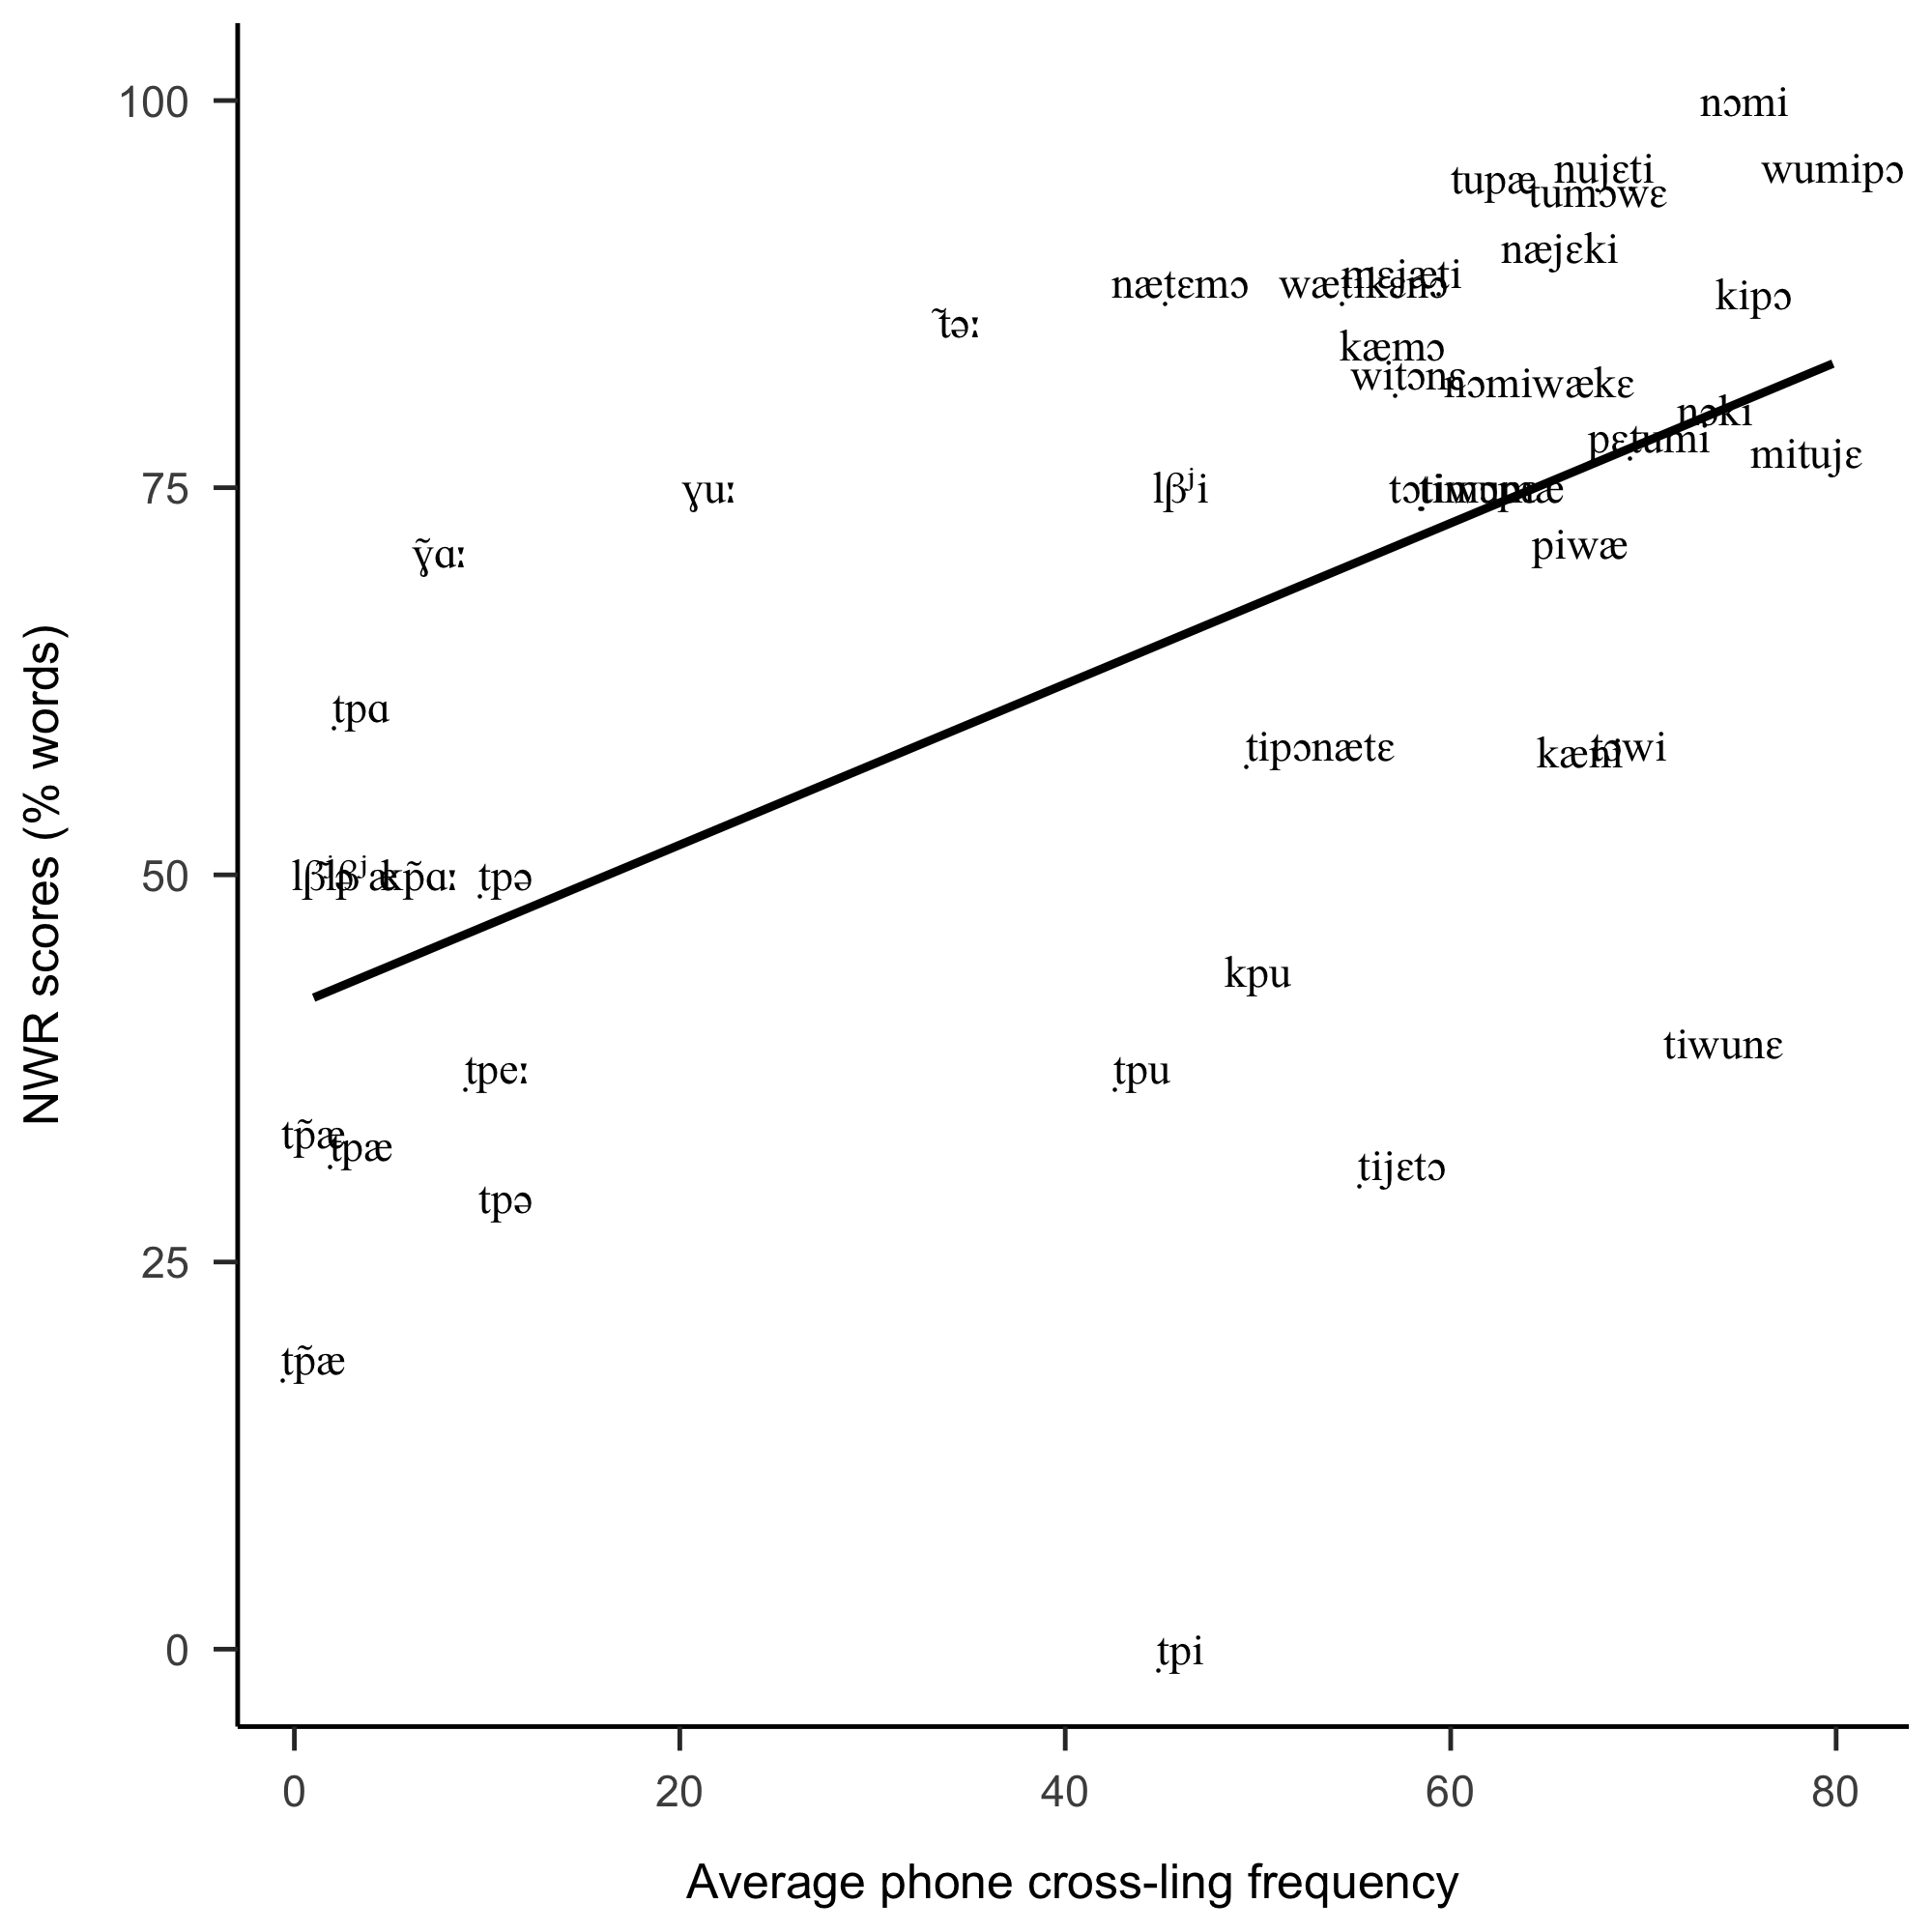
\includegraphics[width=0.65\linewidth]{nwr.by.freq.ITEM} 

}

\caption{NWR scores for individual target words as a function of the average frequency with which each phone is found across languages.}\label{fig:fig-xling-freq}
\end{figure}

Additionally, the effect for the interaction between the two fixed effects was small but significant (ß = 0.22, SE ß = 0.09, p = 0.01): The effect of frequency was larger for older children. Inspection of Figure \ref{fig:fig-xling-freq-age3} suggests that the age effects are more marked for items containing cross-linguistically common phones, such that children's average performance increases more rapidly with age for those than for items containing cross-linguistically uncommon phones.

\begin{figure}[!t]

{\centering \includegraphics[width=0.65\linewidth]{manuscript_files/figure-latex/fig-xling-freq-age3-1} 

}

\caption{NWR scores as a function of age and typological frequency. Lines are fits from the model in the main text predicting NWR scores from child age (x axis) and the average frequency with which each phone is found across languages (mean, or plus/minus one standard deviation). Each circle indicates the estimated NWR scores for one child at one frequency level.}\label{fig:fig-xling-freq-age3}
\end{figure}

\hypertarget{nwr-and-typology-nwr-as-a-function-of-within-language-phone-frequency}{%
\subsubsection{NWR and typology: NWR as a function of within-language phone frequency}\label{nwr-and-typology-nwr-as-a-function-of-within-language-phone-frequency}}

We next checked whether the association between whole-item NWR scores and cross-linguistic phone frequency could actually be due to frequency of the sounds within the language: The same perception and production pressures that shape languages diachronically could affect a language's lexicon, so that sounds that are easier to perceive or produce are more frequent within a language than those that are harder. If so, children will have more experience with the easier sounds, and they may thus be better able to represent and repeat non-words containing them simply because of the additional exposure.

Phone corpus-based frequencies were correlated with phone cross-linguistic frequencies {[}r(27)=0.50, p \textless{} 0.01{]}; and item-level average phone corpus-based frequencies were correlated with the corresponding cross-linguistic frequencies {[}r(38)=0.73, p \textless{} 0.001{]}. Moreover, averaging across participants, the Pearson correlation between scaled average corpus phone frequency and whole-item NWR scores was r(38)=.432, p \textless{} 0.01. Therefore, we fit another mixed logistic regression, this time declaring as fixed effects both scaled cross-linguistic and corpus frequencies (averaged across all attested phones within each stimulus item), in addition to age. As before, the model contained random slopes for both child ID and target. In this model, both cross-linguistic phone frequency (ß = 0.78, SE ß = 0.27, p \textless{} 0.01) and age (ß = 0.35, SE ß = 0.13, p \textless{} 0.01) were significant predictors of whole-item NWR scores, but corpus phone frequency (ß = 0.00, SE ß = 0.25, p = 0.99) was not.

\hypertarget{follow-up-analyses-patterns-in-nwr-mispronunciations}{%
\subsubsection{Follow-up analyses: Patterns in NWR mispronunciations}\label{follow-up-analyses-patterns-in-nwr-mispronunciations}}

We addressed our first research question in a second way, by investigating patterns of error. Unlike all other analyses, we looked at all attempts, so as to base our generalizations on more data. As in all analyses, we did not exclude errors resulting in real words. Deletions were very rare (insertion and metathesis were not attested): there were only 17 instances of deleted vowels (\textasciitilde0.35\% of all vowel targets), and 13 instances of deleted consonants (\textasciitilde0.50\% of all consonant targets). We therefore focus our qualitative description here on substitutions: There were 813 cases of substitutions, \textasciitilde16.81 of the 4836 phones found collapsing across all children and target words, so that substitutions constituted the majority of incorrect phones (\textasciitilde96.10\% of unmatched phones). To inform our understanding of how cross-linguistic patterns may be reflected in NWR scores, we asked: Is it the case that cross-linguistically less common and/or more complex phones are more frequently mispronounced, and more frequently substituted by more common ones than vice versa?\footnote{Note that tables of errors including child age are provided in the project repository for those interested in a finer-grained analysis than what is presented here. See \url{https://osf.io/5qspb/wiki/home/}, quick links, error tables.}

\begin{table}

\caption{\label{tab:tab-v}Number (and percent) of vowel targets that were correctly repeated (Corr.), deleted (Del.), or substituted, as a function of vowel type, and whether the error resulted in a nasality change (Nasal Err.) or only a quality change (Qual. Err.)}
\centering
\begin{tabular}[t]{lrrrrrrrr}
\toprule
  & Corr. & Del. & Nasal Err. & Qual. Err & \% Corr. & \% Del. & \% Nasal Err. & \% Qual Err.\\
\midrule
Nasal Target & 101 & 0 & 39 & 17 & 64.3 & 0.0 & 24.8 & 10.8\\
Oral Target & 1988 & 17 & 52 & 204 & 87.9 & 0.8 & 2.3 & 9.0\\
\bottomrule
\end{tabular}
\end{table}

We looked for potential asymmetries in errors for different types of sounds in vowels by looking at the proportion of vowel phones that were correctly repeated or not, generating separate estimates for nasal and oral vowels. The nasal vowels in our stimuli occur in \textasciitilde1.40\% of languages' phonologies (range 0\% to 3\%);
whereas oral vowels in our stimuli occur in \textasciitilde31.55\% of languages' phonologies (range 3\% to 92\%).
As noted above, frequency within the language is correlated with cross-linguistic frequency, and thus these two types of sounds also differ in the former: Their frequencies in Yélî Dnye are: nasal vowels \textasciitilde0.03‰ (range 0.00‰ to 0.05‰) versus oral \textasciitilde0.23‰ (range 0.02‰ to 0.76‰).

We distinguished errors that included a change of nasality (and may or may not have preserved quality), versus those that preserved nasality (and were therefore a quality error), shown in Table \ref{tab:tab-v}. We found that errors involving nasal vowel targets were more common than those involving oral vowels (35.70 versus 12.10\%). Additionally, errors in which a nasal vowel lost its nasal character were 10 times more common than those in which an oral vowel was produced as a nasal one. Note that this analysis does not tell us whether cross-linguistic or within-language frequency is the best predictor, an issue to which we return below.

\begin{table}

\caption{\label{tab:tab-c}Number (and percent) of consonant targets that were correctly repeated (Corr.), deleted (Del.), or substituted, as a function of the complexity of the consonant, and whether the error resulted in a change of complexity (Cmpl Err.) or not (Othr Err.)}
\centering
\begin{tabular}[t]{lrrrrrrrr}
\toprule
  & Corr. & Del. & Cmpl Err. & Othr Err. & \% Corr. & \% Del & \% Cmpl Err. & \% Othr Err.\\
\midrule
Complex Target & 198 & 0 & 219 & 44 & 43.0 & 0.0 & 47.5 & 9.5\\
Simple Target & 1482 & 13 & 3 & 117 & 91.8 & 0.8 & 0.2 & 7.2\\
\bottomrule
\end{tabular}
\end{table}

For consonants, we inspected complex ({[}ṭp{]}, {[}tp{]}, {[}kp{]}, {[}km{]}, {[}kṇ{]}, {[}mp{]}, and {[}lβʲ{]}) versus simpler ones ({[}m{]}, {[}n{]}, {[}l{]}, {[}w{]}, {[}j{]}, {[}w{]}, {[}ṭ{]}, {[}g{]}, {[}p{]}, {[}t{]}, {[}k{]}, {[}f{]}, {[}ɣ{]}, {[}h{]}, and {[}tʃ{]}), using the same logic: We looked at correct phone repetition, substitution with a change in complexity category, or a change within the same complexity category.\footnote{Note that the substitutions included phones that are not native to Yélî Dnye but do occur in English (e.g., {[}tʃ{]}). These data come from careful transcriptions by a native Yélî Dnye speaker who is very fluent in English.}
The complex consonants in our stimuli occur in \textasciitilde17.33\% of languages' phonologies (range 0\% to 78\%);
whereas simple consonants in our stimuli occur in \textasciitilde67.62\% of languages' phonologies (range 13\% to 96\%).
Again these groups of sounds differ in their frequency within the language. Their type frequencies in Yélî Dnye are: complex consonants \textasciitilde0.04‰ (range 0.00‰ to 0.10‰) versus simple consonants \textasciitilde0.32‰ (range 0.06‰ to 0.55‰).

Table \ref{tab:tab-c} showed that errors involving complex consonant targets were more common than those involving simple consonants (57 versus 8.20\%). Additionally, errors in which a complex consonant was mispronounced as a simple consonant were quite common, whereas those in which a simple consonant was produced as a complex one were vanishingly rare.

To address whether errors were better predicted by cross-linguistic or within-language frequency, we calculated a proportion of productions that were correct for each phone (regardless of the type of error or the substitution pattern). Graphical investigation suggested that in both cases the relationship was monotonic and not linear, so we computed Spearman's rank correlations between the correct repetition score, on the one hand, and the two possible predictors on the other. Although we cannot directly test the interaction due to collinearity, the correlation with cross-linguistic frequency {[}r(346.78)=0.74, p \textless{} 0.001{]} was greater than that with within-language frequency {[}r(817.23)=0.39, p = 0.09{]}.

\hypertarget{length-effects-on-nwr-1}{%
\subsubsection{Length effects on NWR}\label{length-effects-on-nwr-1}}

We next turned to our second research question by inspecting whether NWR scores varied as a function of word length (Table \ref{tab:tablength}). In this section and all subsequent ones, we only look at first attempts, for the reasons discussed previously. Additionally, we noticed that participants scored much lower on monosyllables than on non-words of other lengths. This is likely due to the fact that the majority of monosyllables were designed to include sounds that are rare in the world's languages, which may be harder to produce or perceive, as suggested by our previous analyses of NWR scores as a function of cross-linguistic phone frequency and error patterns. Therefore, we set monosyllables aside for this analysis.

We observed the typical pattern of lower scores for longer items only for the whole-item scoring, and even there differences were rather small. In a generalized binomial mixed model excluding monosyllables, we included 479 observations, from 40 children producing, in any given trial, one of 24 (non-monosyllabic) potential target words. The analysis revealed a positive effect of age (ß = 0.56, SE ß = 0.14, p \textless{} 0.001) and a negative but non-significant estimate for target length in number of syllables (ß = -0.15, SE ß = 0.33, p = 0.65).

\begin{table}

\caption{\label{tab:tablength}NWR means (and standard deviations) measured in whole-word scores and normalized Levenshtein Distance (NLD), separately for the four stimuli lengths.}
\centering
\begin{tabular}[t]{lll}
\toprule
  & Word & NLD\\
\midrule
1 syll & 48 (22) & 40 (18)\\
2 syll & 79 (22) & 8 (9)\\
3 syll & 78 (19) & 7 (7)\\
4 syll & 74 (32) & 9 (12)\\
\bottomrule
\end{tabular}
\end{table}

\hypertarget{individual-variation-and-nwr}{%
\subsubsection{Individual variation and NWR}\label{individual-variation-and-nwr}}

\begin{figure}
\centering
\includegraphics{manuscript_files/figure-latex/fig-scores-by-age-1.pdf}
\caption{\label{fig:fig-scores-by-age}NWR whole-item scores for individual participants as a function of age and sex (purple crosses = boys, orange circles = girls).}
\end{figure}

Our final exploratory analysis assessed whether variation in scores was structured by factors that vary across individuals, as per our third research question. As shown in Figure \ref{fig:fig-scores-by-age}, there was a greater deal of variance across the tested age range, with significantly higher NWR scores for older children (Spearman's rank correlation, given inequality of variance): ρ(38) = .47, p \textless{} 0.01. In contrast, there was no clear association between NWR scores and sex: Welch t (27.33) = -0.60, p = 0.56; NWR scores and birth order (data missing for 14 children): ρ(24) = -.198, p = 0.33; or NWR scores and maternal education: ρ(38) = .097, p = 0.55.

\hypertarget{discussion}{%
\subsection{Discussion}\label{discussion}}

We used non-word repetition to investigate phonological development in a language with a large phonological inventory (including some typologically rare segments). We aimed to provide additional data on two questions already visited in NWR work, namely the influence of stimulus length and individual variation, plus one research area that has received less attention, regarding the possible correlation between typological phone frequency and NWR scores. An additional overarching goal was to discuss NWR in the context of population and language diversity, since it is very commonly used to document phonological development in children raised in urban settings with wide-spread literacy, and has been seldom used in non-European languages (but note there are exceptions, including work cited in the Introduction and in the Discussion below). We consider implications of our results on each of these four research areas in turn.

\hypertarget{nwr-and-typology-1}{%
\subsubsection{NWR and typology}\label{nwr-and-typology-1}}

Arguably the most innovative aspect of our data relate to the inclusion of phones that are less commonly found across languages, and rarely used in NWR tasks. As explained in the Introduction, typological frequency of phones could reflect ease of perception, ease of production, and other factors, and these factors could affect speech processing and production. This predicts a correlation between typological frequency and NWR performance, due to those factors affecting both. To assess this prediction, we looked at our data in two ways. First, we measured the degree of association between NWR scores and cross-linguistic frequency at the level of non-word items. Second, we described mispronunciation patterns, by looking at correct and incorrect repetitions of simpler and more complex sounds, which are also more or less frequent.

There are some reasons to believe that Yélî Dnye put that hypothesis to a critical test: The phoneme inventory is both large and acoustically packed, in addition to containing several typologically infrequent (or unique) contrasts. One could then predict that correlations with typological frequency should be relatively weak because the ambient language puts more pressure on Yélî children to distinguish (perceptually and articulatorily) fine-grained phonetic differences than what is required of child speakers of other languages. On the other hand, it is also possible that this pressure gives Yélî children no benefit, and that some of these categories are simply acquired later in development. We can draw a parallel with children learning another Papuan language, Ku Waru, which has a packed inventory of lateral consonants; children do not produce adult-like realizations of the more complex of these laterals (the pre-stopped velar lateral /ɡ͡ʟ/) until 5 or 6 years of age (Rumsey, 2017).

We do not have the necessary data to assess whether the correlation is indeed weaker for Yélî Dnye learners than learners of other languages, but we did find a robust correlation of average segmental cross-linguistic frequency and NWR performance: Even accounting for age and random effects of item and participant, we saw that target words with typologically more common segments were repeated correctly more often. This effect was large, with a magnitude more than twice the size of the effect of participant age. Additionally, we observed an interaction between age and this factor, which emerged because cross-linguistic frequency explained more variance at older ages (i.e., the difference in performance for more versus less typologically frequent sounds was greater for older than younger children). Importantly, the correlation between performance and typological frequency remained significant after accounting for the frequencies of these segments in a conversational corpus. An analysis of the substitutions made by children also aligned with this interpretation, with typologically more common sounds being substituted for typologically less common ones.

We thus at present conclude that typological frequency of sounds is, to a certain extent, mirrored in children's NWR, in ways that may not be due merely to how often those sounds are used in the ambient language, and which are not erased by language-specific pressure to make finer-grained differences early in development. We do not aim to reopen a debate on the extent to which cross-linguistic frequency of occurrence can be viewed necessarily as reflecting ease of perception or production (via phonotactic constraints, ambiguous parsing conditions, individual differences, and more as in, e.g., Beddor, 2009; Bermúdez-Otero, 2015; Maddieson, 2009; Ohala, 1981; Yu, 2021), but we do point out that this association is interestingly different from effects found in artificial language learning tasks (see Moreton \& Pater, 2012 for a review) which are in some ways quite similar to NWR. We believe that it may be insightful to extend the purview of NWR from a narrow focus on working memory and structural factors to broader uses, including for describing the phonological representations in the perception-production loop (as in e.g., Edwards, Beckman, \& Munson, 2004).

\hypertarget{length-effects-and-nwr}{%
\subsubsection{Length effects and NWR}\label{length-effects-and-nwr}}

We investigated the effect of item complexity on NWR scores by varying the number of syllables in the item. In broad terms, children should have higher NWR scores for shorter items. That said, previous work summarized in the Introduction has shown both very small (e.g., Piazzalunga et al., 2019) and very large (e.g., Cristia et al., 2020) effects of stimulus length. Setting aside our monosyllabic stimuli (which contained typologically infrequent segments with lower NWR scores, as just discussed), we examined effects of item length among the remaining stimuli, which range between 2 and 4 syllables long. The effect of item length was not significant in a statistical model that additionally accounted for age and random effects of item and participant. We do not have a good explanation for why samples in the literature vary so much in terms of the size of length effects, but two possibilities are that this is not truly a length effect but a confound with some other aspect of the stimuli, or that there is variation in phonological representations that is poorly understood. We explain each idea in turn.

First, it remains possible that apparent length effects are actually due to uncontrolled aspects of the stimuli. For instance, some NWR researchers model their non-words on existing words, by changing some vowels and consonants, which could lead to fewer errors (since children have produced similar words in the past); some researchers control tightly the diphone frequency of sub-sequences in the non-words. Building on these two aspects that researchers often control, one can imagine that longer items have fewer neighbors, and thus both the frequency with which children have produced similar items and (relatedly) their n-phone frequency is overall lower. If this idea is correct, a careful analysis of non-words used in previous work may reveal that studies with larger length effects just happened to have longer non-words with lower n-phone frequencies.

Second, NWR is often described as a task that tests flexible perception-production, and as such it is unclear why length effects should be observed at all. However, it is possible that NWR relies on more specific aspects of perception-production, in ways that are dependent on stimulus length. A hint in this direction comes from work on illiterate adults, who can be extremely accurate when repeating short non-words, but whose NWR scores are markedly lower for longer items. In a longitudinal study on Portuguese-speaking adults who were learning to read, Kolinsky, Leite, Carvalho, Franco, and Morais (2018) found that, before reading training, the group scored 12.5\% on 5-syllable items, whereas after 3 months of training, they scored 62.5\% on such long items, whereas performance was at 100\% for monosyllables throughout. Given that as adults they had fully acquired their native language, and obviously they had flexible perception-production schemes that allowed them to repeat new monosyllables perfectly, the change that occurred in those three months must relate to something else in their phonological skills, something that is not essential to speak a language natively. Thus, we hazard the hypothesis that sample differences in length effects may relate to such non-essential skills. Since as stated this hypothesis is under-specified, further conceptual and empirical work is needed.

\hypertarget{individual-variation-and-nwr-1}{%
\subsubsection{Individual variation and NWR}\label{individual-variation-and-nwr-1}}

Our review of previous work in the Introduction suggested that our anticipated sample size would not be sufficient to detect most individual differences using NWR. We give a brief overview of individual difference patterns of four types in the present data---age, sex, birth order, and maternal education---hoping that these findings can contribute to future meta- or mega-analytic efforts aggregating over studies.

In broad terms, we expected that NWR scores would increase with participant age, as this is the pattern observed in several previous studies (English Vance et al., 2005; Italian Piazzalunga et al., 2019; Cantonese Stokes et al., 2006; but not in Cristia et al., 2020). Indeed, age was significantly correlated with NWR scores and it also showed up as a significant predictor of NWR score when included as a control factor in the analyses of both item length and average segmental frequency. In brief, our results underscore the idea that phonological development continues well past the first few years of life, extending into middle childhood and perhaps later (Hazan \& Barrett, 2000; Rumsey, 2017).

In contrast, previous work varies with respect to correlations of NWR scores with maternal education (e.g., Farmani et al., 2018; Kalnak et al., 2014; Meir \& Armon-Lotem, 2017). We did not expect large correlations with maternal education in our sample for two reasons: First, education on Rossel Island is generally highly valued and so widespread that little variation is seen there; second, formal education is not at all essential to ensuring one's success in society and may not be a reliable index of local socioeconomic variation locally. In fact, maternal education correlated with NWR score at about r\textasciitilde.1, which is small. We find correlations of about that size for participant sex, which is aligned with previous work (Chiat \& Roy, 2007).

Finally, we investigated whether birth order might correlate with NWR scores, as it does with other language tasks, such that first-born children showing higher scores on standardized language tests than later-born children (Havron et al., 2019) and adults (in a battery including verbal abilities, e.g., Barclay, 2015), presumably because later-born children receive a smaller share of parental input and attention than first-borns. Given shared caregiving practices and the hamlet organization typical of Rossel communities, children have many sources of adult and older child input that they encounter on a daily basis and first-born children quickly integrate with a much larger pool of both older and younger children with whom they partly share caregivers. Therefore we expected that any correlations with birth order on NWR would be attenuated in this context. In line with this prediction, our descriptive analysis showed a non-significant correlation between birth order and NWR score. However, the effect size was larger than that found for the other two factors and it is far from negligible, at r\textasciitilde.2 or Cohen's d\textasciitilde0.41. In fact, two large studies (with therefore precise estimates) found effects of about d\textasciitilde.2 for birth order effects on other language tasks (Barclay, 2015; Havron et al., 2019), which would suggest the correlations we found are larger. We therefore believe it may be worth revisiting this question with larger samples in similar child-rearing environments, to further assess whether distributed child care results in more even language outcomes for first- and later-born children.

\hypertarget{nwr-across-languages-and-cultures}{%
\subsubsection{NWR across languages and cultures}\label{nwr-across-languages-and-cultures}}

The fourth research area to which we wanted to contribute pertained to the use of NWR across languages and populations, since when designing this study we wondered whether NWR was a \emph{culture-fair} test of phonological development. Although our data cannot answer this question because we have only sampled one language and population here, we would like to spend some time discussing the integration of these results to the wider NWR literature. It is important to note at the outset that we cannot obtain a final answer because integration across studies implies not only variation in languages and child-rearing settings, but also in methodological aspects including non-word length, non-word design (e.g., the syllable and phone complexity included in the items), and task administration, among others. Nonetheless, we feel the NWR task is prevalent enough to warrant discussion about this, similarly to other tasks sometimes used to describe and compare children's language skills across populations, like the recent re-use of the MacArthur-Bates Communicative Development Inventory to look at vocabulary acquisition across multiple languages (Frank et al., 2017).

The range of performance we observed overlapped with previously observed levels of performance. Paired with our thorough training protocol, we had interpreted the NWR scores among Yélî Dnye learners as indicating that our adaptations of NWR for this context were successful, even given a number of non-standard changes to the training phase and to the design of the stimuli. Additionally, it seemed that Yélî children showed comparable performance to others tested on a similar task, despite the many linguistic, cultural, and socioeconomic differences between this and previously tested populations, unlike the case that had been reported for the Tsimane' (Cristia et al., 2020).

Comparison across published studies is difficult (see SM2 for our preliminary attempt). To be certain whether language-specific characteristics do account for meaningful variation in NWR scores, it will be necessary to design NWR tasks that are cross-linguistically valid. We believe this will be exceedingly difficult (or perhaps impossible), since it would entail defining a 10-20 set of items that are meaningless, but phonotactically legal, in all of the languages. An alternative may be to find ways to regress out some of these differences, and thus compare languages while controlling for choices of phonemes, syllable structure, and overall length of the NWR items. Both of these issues are discussed in Chiat (2015). As for the variable strengths of age correlations discussed above, here as well we are uncertain to what they may be due, but we do hope that these intriguing observations will lead others to collect and share NWR data.

\hypertarget{limitations}{%
\subsubsection{Limitations}\label{limitations}}

Before closing, we would like to point out some salient limitations of the current work. To begin with, we only employed one set of non-words, in which not all characteristics that previous work suggest matter were manipulated (Chiat, 2015). As a result, we only have a rather whole-sale measure of performance, and we do not know to what extent lexical knowledge, pure phonological knowledge, and working memory, among others, contribute to children's performance. Similarly, our items varied systematically in length and typological frequency of the sounds included, but not in other potential dimensions (such as whether the items contained morphemes of the language or not).

We relied on a single resource, PHOIBLE, for our estimation of typological frequency, and some readers may be worried about the effects of this choice. As far as we know, PHOIBLE is the most extensive archive of phonological inventories, so it is a reasonable choice in the current context. However, one may want to calculate typological frequency not by trying to have as many languages represented as possible, but rather by selecting a sample of typologically independent languages. In addition, it is not the case that all the world's languages are represented, and indeed some of the Yélî sounds were not found in PHOIBLE. PHOIBLE---as well as our own work---depends on phonological descriptions from linguists who are in many cases not native speakers of the languages. Because the phones in our items have largely been evidenced as phonemic via multiple analyses (i.e., minimal contrast, phonological, phonetic, and ultrasound, see Levinson, 2021), we are not concerned that changes to the phonological description in the future (e.g., if a segment loses its phonemic status) will significantly change the results presented here. Relatedly, any converging evidence from the other ongoing studies of Yélî Dnye phonological development and fine-grained analyses of sound substitutions would certainly help bolster the claims we made here. While all these limitations should be borne in mind, it is important to also consider what our conclusions were, and that is that there is a non-trivial correlation between NWR and typological frequency. At present, we do not see how imbalance in the typological selection and missing data can conspire to produce the correlation we observe. If anything, these factors should increase noise in the typological frequency estimation, in which case the correlation size we uncover is an underestimation of the true correlation.

Additionally, we only had a single person interacting with children as well as interpreting children's production, so we do not know to what extent our findings generalize to other experimenters and research assistants. Furthermore, since both stimuli presentation and production data collected were audio-only, neither the children nor our research assistant were able to integrate visual production cues in their interpretation. Other work shows that children's performance reaches ceiling by 12 years of age for auditorily-presented minimal pairs for typologically rare (i.e., pre- vs post-alveolar stop) contrasts (Casillas \& Levinson, In preparation). Nonetheless, language processing for the majority of children will be audiovisual in natural conditions, and thus it may be interesting in the future to capture this aspect of speech.

\hypertarget{conclusions}{%
\subsubsection{Conclusions}\label{conclusions}}

The present study shows that NWR can be adapted for very different populations than have previously been tested. In addition, we observed strong correlations with age and typological frequency, while correlations with item length, participant sex, maternal education, and birth order were weaker. A consideration of previous work led us to suggest that the statistical strength of all of these effects may vary depending on the linguistic, cultural, and socio-demographic properties of the population under study, in conjunction with characteristics of the non-word items used. The present findings raise many questions, including: Why do NWR scores pattern differently across samples? What does that tell us about the relationship between lexical development, phonological development, and the input environment? What is implied about the joint applicability of these outcome measures as a diagnostic indicator for language delays and disorders? While answers to these questions should be sought in future work, we take the present findings as robustly supporting the idea that phonological development continues well past early childhood and as yielding preliminary support for a potential association between individual learners' NWR and much broader patterns of cross-linguistic phone frequency.

\newpage

\hypertarget{acknowledgments}{%
\subsection{Acknowledgments}\label{acknowledgments}}

We are grateful to the individuals who participated in the study, and the families and communities that made it possible. The collection and annotation of these recordings was made possible by Ndapw:éé Yidika, Taakêmê Ńamono, and Y:aaw:aa Pikuwa; with thanks also to the PNG National Research Institute, and the Administration of Milne Bay Province. We owe big thanks also to Stephen C. Levinson for his invaluable advice and support and Shawn C. Tice for helpful discussion during data collection. AC acknowledges financial and institutional support from Agence Nationale de la Recherche (ANR-17-CE28-0007 LangAge, ANR-16-DATA-0004 ACLEW, ANR-14-CE30-0003 MechELex, ANR-17-EURE-0017) and the J. S. McDonnell Foundation Understanding Human Cognition Scholar Award. MC acknowledges financial support from an NWO Veni Innovational Scheme grant (275-89-033).

\hypertarget{data-code-and-materials-availability-statement}{%
\subsection{Data, code and materials availability statement}\label{data-code-and-materials-availability-statement}}

All data, code, and materials are available from \url{https://osf.io/5qspb/}

\hypertarget{references}{%
\section{References}\label{references}}

\setlength{\parindent}{-0.5in}
\setlength{\leftskip}{0.5in}

\hypertarget{refs}{}
\begin{CSLReferences}{1}{0}
\leavevmode\vadjust pre{\hypertarget{ref-armon2015assessing}{}}%
Armon-Lotem, S., Jong, J. de, \& Meir, N. (2015). \emph{Methods for assessing multilingual children: Disentangling bilingualism from specific language impairment}. Bristol: Multilingual matters.

\leavevmode\vadjust pre{\hypertarget{ref-balladares2016socio}{}}%
Balladares, J., Marshall, C., \& Griffiths, Y. (2016). {Socio-economic status affects sentence repetition, but not non-word repetition, in Chilean preschoolers}. \emph{{First Language}}, \emph{36}(3), 338--351. \url{https://doi.org/10.1177/0142723715626067}

\leavevmode\vadjust pre{\hypertarget{ref-barclay2015within}{}}%
Barclay, K. J. (2015). A within-family analysis of birth order and intelligence using population conscription data on {S}wedish men. \emph{Intelligence}, \emph{49}, 134--143.

\leavevmode\vadjust pre{\hypertarget{ref-beddor2009coarticulatory}{}}%
Beddor, P. S. (2009). A coarticulatory path to sound change. \emph{Language}, \emph{85}(4), 785--832.

\leavevmode\vadjust pre{\hypertarget{ref-bermudezotero2015amphichronic}{}}%
Bermúdez-Otero, R. (2015). Amphichronic explanation and the life cycle of phonological processes. In P. Honeybone \& J. Salmons (Eds.), \emph{The {O}xford handbook of historical phonology} (pp. 374--399). Oxford, UK: Oxford University Press.

\leavevmode\vadjust pre{\hypertarget{ref-Praat}{}}%
Boersma, P., \& Weenink, D. (2020). Praat: Doing phonetics by computer (Version 6.1.35). Retrieved from \url{http://www.praat.org/}

\leavevmode\vadjust pre{\hypertarget{ref-bowey2001nonword}{}}%
Bowey, J. A. (2001). Nonword repetition and young children's receptive vocabulary: A longitudinal study. \emph{Applied Psycholinguistics}, \emph{22}(3), 441--469.

\leavevmode\vadjust pre{\hypertarget{ref-brandeker2015language}{}}%
Brandeker, M., \& Thordardottir, E. (2015). Language exposure in bilingual toddlers: Performance on nonword repetition and lexical tasks. \emph{American Journal of Speech-Language Pathology}, \emph{24}(2), 126--138.

\leavevmode\vadjust pre{\hypertarget{ref-brown2011cultural}{}}%
Brown, P. (2011). The cultural organization of attention. In A. Duranti, E. Ochs, \& and Bambi B Schieffelin (Eds.), \emph{Handbook of {Language Socialization}} (pp. 29--55). Malden, MA: Wiley-Blackwell.

\leavevmode\vadjust pre{\hypertarget{ref-brown2014interactional}{}}%
Brown, P. (2014). The interactional context of language learning in {T}zeltal. In I. Arnon, M. Casillas, C. Kurumada, \& B. Estigarribia (Eds.), \emph{Language in interaction: Studies in honor of {Eve V. Clark}} (pp. 51-\/-82). Amsterdam, NL: John Benjamins.

\leavevmode\vadjust pre{\hypertarget{ref-brownIPchildrearing}{}}%
Brown, P., \& Casillas, M. (in press). Childrearing through social interaction on {Rossel Island, PNG}. In A. J. Fentiman \& M. Goody (Eds.), \emph{{Esther Goody} revisited: Exploring the legacy of an original inter-disciplinarian} (pp. XX--XX). New York, NY: Berghahn.

\leavevmode\vadjust pre{\hypertarget{ref-bunceURcrosscultural}{}}%
Bunce, J., Soderstrom, M., Bergelson, E., Rosemberg, C., Stein, A., Alam, F., \ldots{} Casillas, M. (under review). A cross-cultural examination of young children's everyday language experiences.

\leavevmode\vadjust pre{\hypertarget{ref-casillas2021early}{}}%
Casillas, M., Brown, P., \& Levinson, S. C. (2021). {Early language experience in a Papuan community}. \emph{Journal of Child Language}, \emph{48}(4), 792--814.

\leavevmode\vadjust pre{\hypertarget{ref-casillasIPmarkedness}{}}%
Casillas, M., \& Levinson, S. C. (In preparation). Markedness and minimal pair discrimination in children learning {Yélî Dnye}.

\leavevmode\vadjust pre{\hypertarget{ref-castro1998illiterate}{}}%
Castro-Caldas, A., Petersson, K. M., Reis, A., Stone-Elander, S., \& Ingvar, M. (1998). {The illiterate brain. Learning to read and write during childhood influences the functional organization of the adult brain.} \emph{Brain: A Journal of Neurology}, \emph{121}(6), 1053--1063. \url{https://doi.org/10.1093/brain/121.6.1053}

\leavevmode\vadjust pre{\hypertarget{ref-chiat2015nonword}{}}%
Chiat, S. (2015). Non-word repetition. In S. Armon-Lotem, J. de Jong, \& N. Meir (Eds.), \emph{Methods for assessing multilingual children: Disentangling bilingualism from specific language impairment} (pp. 125--150). Bristol: Multilingual matters.

\leavevmode\vadjust pre{\hypertarget{ref-chiat2007preschool}{}}%
Chiat, S., \& Roy, P. (2007). The preschool repetition test: An evaluation of performance in typically developing and clinically referred children. \emph{Journal of Speech, Language, and Hearing Research}, \emph{50}(2), 429--443.

\leavevmode\vadjust pre{\hypertarget{ref-coady2008uses}{}}%
Coady, J. A., \& Evans, J. L. (2008). Uses and interpretations of non-word repetition tasks in children with and without specific language impairments (SLI). \emph{International Journal of Language \& Communication Disorders}, \emph{43}(1), 1--40.

\leavevmode\vadjust pre{\hypertarget{ref-is08042009language}{}}%
COST Action. (2009). Language impairment in a multilingual society: Linguistic patterns and the road to assessment. \emph{Brussels: COST Office. Available Online at: Http://Www.bi-Sli.org}.

\leavevmode\vadjust pre{\hypertarget{ref-cristia2021supplementary}{}}%
Cristia, A., \& Casillas, M. (2021). Supplementary materials to non-word repetition in children learning {Yélî D}nye. Retrieved from \url{https://osf.io/5qspb/wiki/home/}

\leavevmode\vadjust pre{\hypertarget{ref-cristia2020infant}{}}%
Cristia, A., Farabolini, G., Scaff, C., Havron, N., \& Stieglitz, J. (2020). Infant-directed input and literacy effects on phonological processing: Non-word repetition scores among the {T}simane'. \emph{PLoS ONE}, \emph{15}(9), e0237702. https://doi.org/\url{https://doi.org/10.1371/journal.pone.0237702}

\leavevmode\vadjust pre{\hypertarget{ref-edwards2004interaction}{}}%
Edwards, J., Beckman, M. E., \& Munson, B. (2004). The interaction between vocabulary size and phonotactic probability effects on children's production accuracy and fluency in nonword repetition. \emph{Journal of Speech, Language, and Hearing Research}, \emph{47}, 421--436.

\leavevmode\vadjust pre{\hypertarget{ref-estes2007differences}{}}%
Estes, K. G., Evans, J. L., \& Else-Quest, N. M. (2007). Differences in the nonword repetition performance of children with and without specific language impairment: A meta-analysis. \emph{Journal of Speech, Language, and Hearing Research}, \emph{50}, 177--195.

\leavevmode\vadjust pre{\hypertarget{ref-farabolini2021nonword}{}}%
Farabolini, G., Rinaldi, P., Caselli, C., \& Cristia, A. (2021). Non-word repetition in bilingual children: The role of language exposure, vocabulary scores and environmental factors. \emph{Speech Language and Hearing}, 1--16. \url{https://doi.org/10.1080/2050571X.2021.1879609}

\leavevmode\vadjust pre{\hypertarget{ref-farabolini2021association}{}}%
Farabolini, G., Taboh, A., Ceravolo, M. G., \& Guerra, F. (2021). The association between language exposure and non-word repetition performance in bilingual children: A meta-analysis. \emph{Under Review}.

\leavevmode\vadjust pre{\hypertarget{ref-farmani2018normalization}{}}%
Farmani, H., Sayyahi, F., Soleymani, Z., Labbaf, F. Z., Talebi, E., \& Shourvazi, Z. (2018). Normalization of the non-word repetition test in {F}arsi-speaking children. \emph{Journal of Modern Rehabilitation}, \emph{12}(4), 217--224.

\leavevmode\vadjust pre{\hypertarget{ref-foley1986papuan}{}}%
Foley, W. A. (1986). \emph{{The Papuan languages of New Guinea}}. Cambridge, UK: Cambridge University Press.

\leavevmode\vadjust pre{\hypertarget{ref-frank2017wordbank}{}}%
Frank, M. C., Braginsky, M., Yurovsky, D., \& Marchman, V. A. (2017). Wordbank: An open repository for developmental vocabulary data. \emph{Journal of Child Language}, \emph{44}(3), 677--694.

\leavevmode\vadjust pre{\hypertarget{ref-gallagher2014identity}{}}%
Gallagher, G. (2014). {An identity bias in phonotactics: Evidence from Cochabamba Quechua}. \emph{Laboratory Phonology}, \emph{5}(3), 337--378. \url{https://doi.org/10.1515/lp-2014-0012}

\leavevmode\vadjust pre{\hypertarget{ref-gathercole1991differentiating}{}}%
Gathercole, S. E., Willis, C., \& Baddeley, A. D. (1991). Differentiating phonological memory and awareness of rhyme: Reading and vocabulary development in children. \emph{British Journal of Psychology}, \emph{82}(3), 387--406.

\leavevmode\vadjust pre{\hypertarget{ref-gratz2018competition}{}}%
Grätz, M. (2018). Competition in the family: Inequality between siblings and the intergenerational transmission of educational advantage. \emph{Sociological Science}, \emph{5}, 246--269.

\leavevmode\vadjust pre{\hypertarget{ref-havron2019effect}{}}%
Havron, N., Ramus, F., Heude, B., Forhan, A., Cristia, A., Peyre, H., \& Group, E. M.-C. C. S. (2019). The effect of older siblings on language development as a function of age difference and sex. \emph{Psychological Science}, \emph{30}(9), 1333--1343.

\leavevmode\vadjust pre{\hypertarget{ref-hazan2000development}{}}%
Hazan, V., \& Barrett, S. (2000). The development of phonemic categorization in children aged 6--12. \emph{Journal of Phonetics}, \emph{28}(4), 377--396.

\leavevmode\vadjust pre{\hypertarget{ref-hellwigPAlanguage}{}}%
Hellwig, B., Sarvasy, H., \& Casillas, M. (provisionally accepted). Language acquisition. In N. Evans \& S. Fedden (Eds.), \emph{The {O}xford guide to {P}apuan languages} (pp. XX--XX). Oxford: Oxford University Press.

\leavevmode\vadjust pre{\hypertarget{ref-jabere2018xperiment}{}}%
Jaber-Awida, A. (2018). Experiment in non word repetition by monolingual {A}rabic preschoolers. \emph{Athens Journal of Philology}, \emph{5}, 317--334. \url{https://doi.org/10.30958/ajp.5-4-4}

\leavevmode\vadjust pre{\hypertarget{ref-kalnak2014nonword}{}}%
Kalnak, N., Peyrard-Janvid, M., Forssberg, H., \& Sahlén, B. (2014). Nonword repetition--a clinical marker for specific language impairment in {S}wedish associated with parents' language-related problems. \emph{PloS One}, \emph{9}(2), e89544.

\leavevmode\vadjust pre{\hypertarget{ref-kolinsky2018completely}{}}%
Kolinsky, R., Leite, I., Carvalho, C., Franco, A., \& Morais, J. (2018). Completely illiterate adults can learn to decode in 3 months. \emph{Reading and Writing}, \emph{31}(3), 649--677. \url{https://doi.org/10.1007/s11145-017-9804-7}

\leavevmode\vadjust pre{\hypertarget{ref-lancy2015anthropology}{}}%
Lancy, D. F. (2015). \emph{The anthropology of childhood}. Cambridge, UK: Cambridge University Press.

\leavevmode\vadjust pre{\hypertarget{ref-lehmann2018early}{}}%
Lehmann, J.-Y. K., Nuevo-Chiquero, A., \& Vidal-Fernandez, M. (2018). The early origins of birth order differences in children's outcomes and parental behavior. \emph{Journal of Human Resources}, \emph{53}(1), 123--156.

\leavevmode\vadjust pre{\hypertarget{ref-levinsonYDgrammar}{}}%
Levinson, S. C. (2021). \emph{A grammar of {Yélî D}nye, the {P}apuan language of {R}ossel {I}sland}. Berlin, Boston: De Gruyter Mouton.

\leavevmode\vadjust pre{\hypertarget{ref-liszkowski2012prelinguistic}{}}%
Liszkowski, U., Brown, P., Callaghan, T., Takada, A., \& de Vos, C. (2012). A prelinguistic gestural universal of human communication. \emph{Cognitive Science}, \emph{36}(4), 698--713. \url{https://doi.org/10.1111/j.1551-6709.2011.01228.x}

\leavevmode\vadjust pre{\hypertarget{ref-maddieson2005correlating}{}}%
Maddieson, I. (2005). Correlating phonological complexity: Data and validation. \emph{UC Berkeley PhonLab Annual Report}, \emph{1}(1).

\leavevmode\vadjust pre{\hypertarget{ref-maddieson2009phonology}{}}%
Maddieson, I. (2009). Phonology, naturalness and universals. \emph{Pozn{á}n Studies in Contemporary Linguistics}, \emph{45}(1), 131--140.

\leavevmode\vadjust pre{\hypertarget{ref-maddieson2013consonant}{}}%
Maddieson, I. (2013a). Consonant inventories. \emph{The World Atlas of Language Structures Online}. Retrieved from \url{https://wals.info/chapter/1}

\leavevmode\vadjust pre{\hypertarget{ref-maddieson2013vowel}{}}%
Maddieson, I. (2013b). Vowel quality inventories. \emph{The World Atlas of Language Structures Online}. Retrieved from \url{https://wals.info/chapter/2}

\leavevmode\vadjust pre{\hypertarget{ref-maddiesonIPphoneticsYD}{}}%
Maddieson, I., \& Levinson, S. C. (in preparation). \emph{The phonetics of {Yélî Dnye}, the language of {Rossel Island}}.

\leavevmode\vadjust pre{\hypertarget{ref-meir2017independent}{}}%
Meir, N., \& Armon-Lotem, S. (2017). Independent and combined effects of socioeconomic status ({SES}) and bilingualism on children's vocabulary and verbal short-term memory. \emph{Frontiers in Psychology}, \emph{8}, 1442.

\leavevmode\vadjust pre{\hypertarget{ref-meir2016disentangling}{}}%
Meir, N., Walters, J., \& Armon-Lotem, S. (2016). {Disentangling SLI and bilingualism using sentence repetition tasks: The impact of L1 and L2 properties}. \emph{International Journal of Bilingualism}, \emph{20}(4), 421--452.

\leavevmode\vadjust pre{\hypertarget{ref-phoible}{}}%
Moran, S., \& McCloy, D. (Eds.). (2019). \emph{PHOIBLE 2.0}. Jena: Max Planck Institute for the Science of Human History. Retrieved from \url{https://phoible.org/}

\leavevmode\vadjust pre{\hypertarget{ref-moreton2012structure}{}}%
Moreton, E., \& Pater, J. (2012). Structure and substance in artificial-phonology learning, part {II}: substance. \emph{Language and Linguistics Compass}, \emph{6}(11), 702--718.

\leavevmode\vadjust pre{\hypertarget{ref-ohala1981listener}{}}%
Ohala, J. J. (1981). The listener as a source of sound change. In M. F. Miller, C. S. Masek, \& R. A. Hendrick (Eds.), \emph{Papers from the parasession on language and behavior} (pp. 178--203). Chicago, IL: Chicago Linguistics Society.

\leavevmode\vadjust pre{\hypertarget{ref-peuteIPconsonants}{}}%
Peute, A. A. K., Fikkert, P., \& Casillas, M. (In preparation). Early consonant production in {Y}élî {D}nye and {T}seltal.

\leavevmode\vadjust pre{\hypertarget{ref-piazzalunga2019articulatory}{}}%
Piazzalunga, S., Previtali, L., Pozzoli, R., Scarponi, L., \& Schindler, A. (2019). {An articulatory-based disyllabic and trisyllabic Non-Word Repetition test: reliability and validity in Italian 3-to 7-year-old children}. \emph{Clinical Linguistics \& Phonetics}, \emph{33}(5), 437--456.

\leavevmode\vadjust pre{\hypertarget{ref-rumsey2017dependency}{}}%
Rumsey, A. (2017). Dependency and relative determination in language acquisition: The case of {Ku Waru}. In N. J. Enfield (Ed.), \emph{Dependencies in language} (pp. 97--116). Berlin: Language Science Press.

\leavevmode\vadjust pre{\hypertarget{ref-dos2020epreuve}{}}%
Santos, C. dos, Frau, S., Labrevoit, S., \& Zebib, R. (2020). L'{é}preuve de r{é}p{é}tition de non-mots LITMUS-NWR-FR {é}value-t-elle la phonologie? In \emph{SHS web of conferences} (Vol. 78, p. 10005). EDP Sciences.

\leavevmode\vadjust pre{\hypertarget{ref-scaff2019}{}}%
Scaff, C. (2019). \emph{Beyond {WEIRD}: An interdisciplinary approach to language acquisition} (PhD thesis).

\leavevmode\vadjust pre{\hypertarget{ref-scaff2021daylong}{}}%
Scaff, C., Stieglitz, J., Casillas, M., \& Cristia, A. (under review). Daylong audio recordings of young children in a forager-farmer society show low levels of verbal input with minimal age-related changes.

\leavevmode\vadjust pre{\hypertarget{ref-stokes2006nonword}{}}%
Stokes, S. F., Wong, A. M., Fletcher, P., \& Leonard, L. B. (2006). Nonword repetition and sentence repetition as clinical markers of specific language impairment: The case of {C}antonese. \emph{Journal of Speech, Language, and Hearing Research}, \emph{49}, 219--236.

\leavevmode\vadjust pre{\hypertarget{ref-torrington2015non}{}}%
Torrington Eaton, C., Newman, R. S., Ratner, N. B., \& Rowe, M. L. (2015). Non-word repetition in 2-year-olds: Replication of an adapted paradigm and a useful methodological extension. \emph{Clinical Linguistics \& Phonetics}, \emph{29}(7), 523--535.

\leavevmode\vadjust pre{\hypertarget{ref-tuller2018identifying}{}}%
Tuller, L., Hamann, C., Chilla, S., Ferré, S., Morin, E., Prevost, P., \ldots{} Zebib, R. (2018). Identifying language impairment in bilingual children in {France and in Germany}. \emph{International Journal of Language \& Communication Disorders}, \emph{53}(4), 888--904.

\leavevmode\vadjust pre{\hypertarget{ref-vance2005speech}{}}%
Vance, M., Stackhouse, J., \& Wells, B. (2005). Speech-production skills in children aged 3--7 years. \emph{International Journal of Language \& Communication Disorders}, \emph{40}(1), 29--48.

\leavevmode\vadjust pre{\hypertarget{ref-wilsenach2013phonological}{}}%
Wilsenach, C. (2013). {Phonological skills as predictor of reading success: An investigation of emergent bilingual Northern Sotho/English learners}. \emph{{Per Linguam: A Journal of Language Learning= Per Linguam: Tydskrif Vir Taalaanleer}}, \emph{29}(2), 17--32. \url{https://doi.org/10.5785/29-2-554}

\leavevmode\vadjust pre{\hypertarget{ref-yu2021toward}{}}%
Yu, A. C. L. (2021). Toward an individual-difference perspective on phonologization. \emph{Glossa: A Journal of General Linguistics}, \emph{6}(1), 1--24.

\end{CSLReferences}


\end{document}
